\documentclass[hyperref=colorlinks]{beamer}
\mode<presentation>
\usetheme{iclpt}
\setbeamertemplate{navigation symbols}{}
\setbeamertemplate{headline}{
  \begin{beamercolorbox}[leftskip=.2cm,rightskip=.2cm,topskip=.2cm,ht=1.1cm,dp=0.1cm,wd=\textwidth]{institute in head/foot}
    
\includegraphics[height=1cm]{icl.pdf}
    \hfill
%    \includegraphics[height=1cm]{../Pics/ATLAS-Logo-Square-Blue-RGB.png}
%    
\includegraphics[height=1cm]{../Pics/CMS-Color.pdf}
    
\includegraphics[height=1cm]{TalkPics/t2k_logo_large.png}

%??put t2k logo here
  \end{beamercolorbox}
}
\setbeamertemplate{footline}{
  \begin{beamercolorbox}[ht=.35cm,dp=0.2cm,wd=\textwidth,leftskip=.3cm]{author in head/foot}%
    \begin{minipage}[c]{5cm}%
      \usebeamerfont{author in head/foot}
      \insertshortauthor 
      \insertshorttitle
    \end{minipage}\hfill%
    \hfill
    \insertframenumber{} / \ref{lastframe}
    %\hfill
    \begin{minipage}{6cm}
      \hfill
      %\insertshorttitle
    \end{minipage}
  \end{beamercolorbox}%
}

\definecolor{beamer@icdarkblue}{RGB}{0,51,102}
\definecolor{beamer@icmiddleblue}{RGB}{0,82,150} 
\definecolor{beamer@iclightblue}{RGB}{200,212,232}
\definecolor{beamer@icmiddlered}{RGB}{204,51,0}
\definecolor{beamer@iclightred}{RGB}{232,212,32}

\usepackage{tikz}
\usetikzlibrary{arrows,shapes,backgrounds,automata}
\usepackage{color}
\usepackage{tabularx,colortbl}
\usepackage{graphicx}
\usepackage{pdfpages}
\usepackage{feynmp}
\usepackage{rotating}
\usepackage{moresize}
\usepackage{slashed}
\usepackage{xcolor,colortbl}
\DeclareGraphicsRule{*}{mps}{*}{}
\hypersetup{colorlinks=false}
\def\checkmark{\tikz\fill[scale=0.4](0,.35) -- (.25,0) -- (1,.7) -- (.25,.15) -- cycle;}

\title[Applications of Computational Physics]{\vspace{-0.2cm} Applications of Computational Physics}
\author[P. Dunne]{Patrick Dunne - Imperial College London}
\titlegraphic{
  \vspace{-0.4cm}
}
\date{}
\begin{document}
\tikzstyle{every picture}+=[remember picture]
\tikzstyle{na} = [baseline=-.5ex]
\begin{fmffile}{t2ktemplatefeyndiags}


  %TITLE PAGE
  %20 mins + 5 questions
  \section{Title}
  \begin{frame}
    \titlepage
  \end{frame}

  \begin{frame}
    \frametitle{Overview}
    \begin{block}{}
        \begin{itemize}
        \item Show applications of the techniques from lectures
        \item Focus on details of implementation in complex high energy physics research situations
        \item[-] Neutrino physics at T2K
        \item[-] Hadron collider physics at CMS
      \end{itemize}
    \end{block}
  \end{frame}

  \begin{frame}
    \frametitle{What do we mean by complex?}
    %ref slide 9 lecture 8 for T2K and CMS number of parameters and datasets for complexity (clarence banff slides from 2 weeks ago (written on 23rd Nov) for massive matrix)    
    \begin{itemize}
    \item Simple examples covered in lectures, e.g. minimising $\chi^{2}$:
    \end{itemize}
    \begin{equation*}
    \chi^{2}(a,\alpha)=\sum_{i=1}^{N^{data}}\frac{\left(d_{i}^{obs}-d_{i}^{model}(a,\alpha)\right)^{2}}{\sigma_{i}^{2}}
    \end{equation*}
    \begin{itemize}
    \item This has uncorrelated errors and a 2 paramter physics model
    \item Plausible that an analytic solution could be found quickly
    \item This will not be the case with applications shown today
    \end{itemize}
  \end{frame}

  \begin{frame}
    \frametitle{T2K}
    \begin{itemize}
    \item Searching for neutrino oscillations in a $\nu_{\mu}/\bar{\nu}_{\mu}$ beam
    \item Looking for matter-antimatter asymmetry in lepton sector
    \end{itemize}
    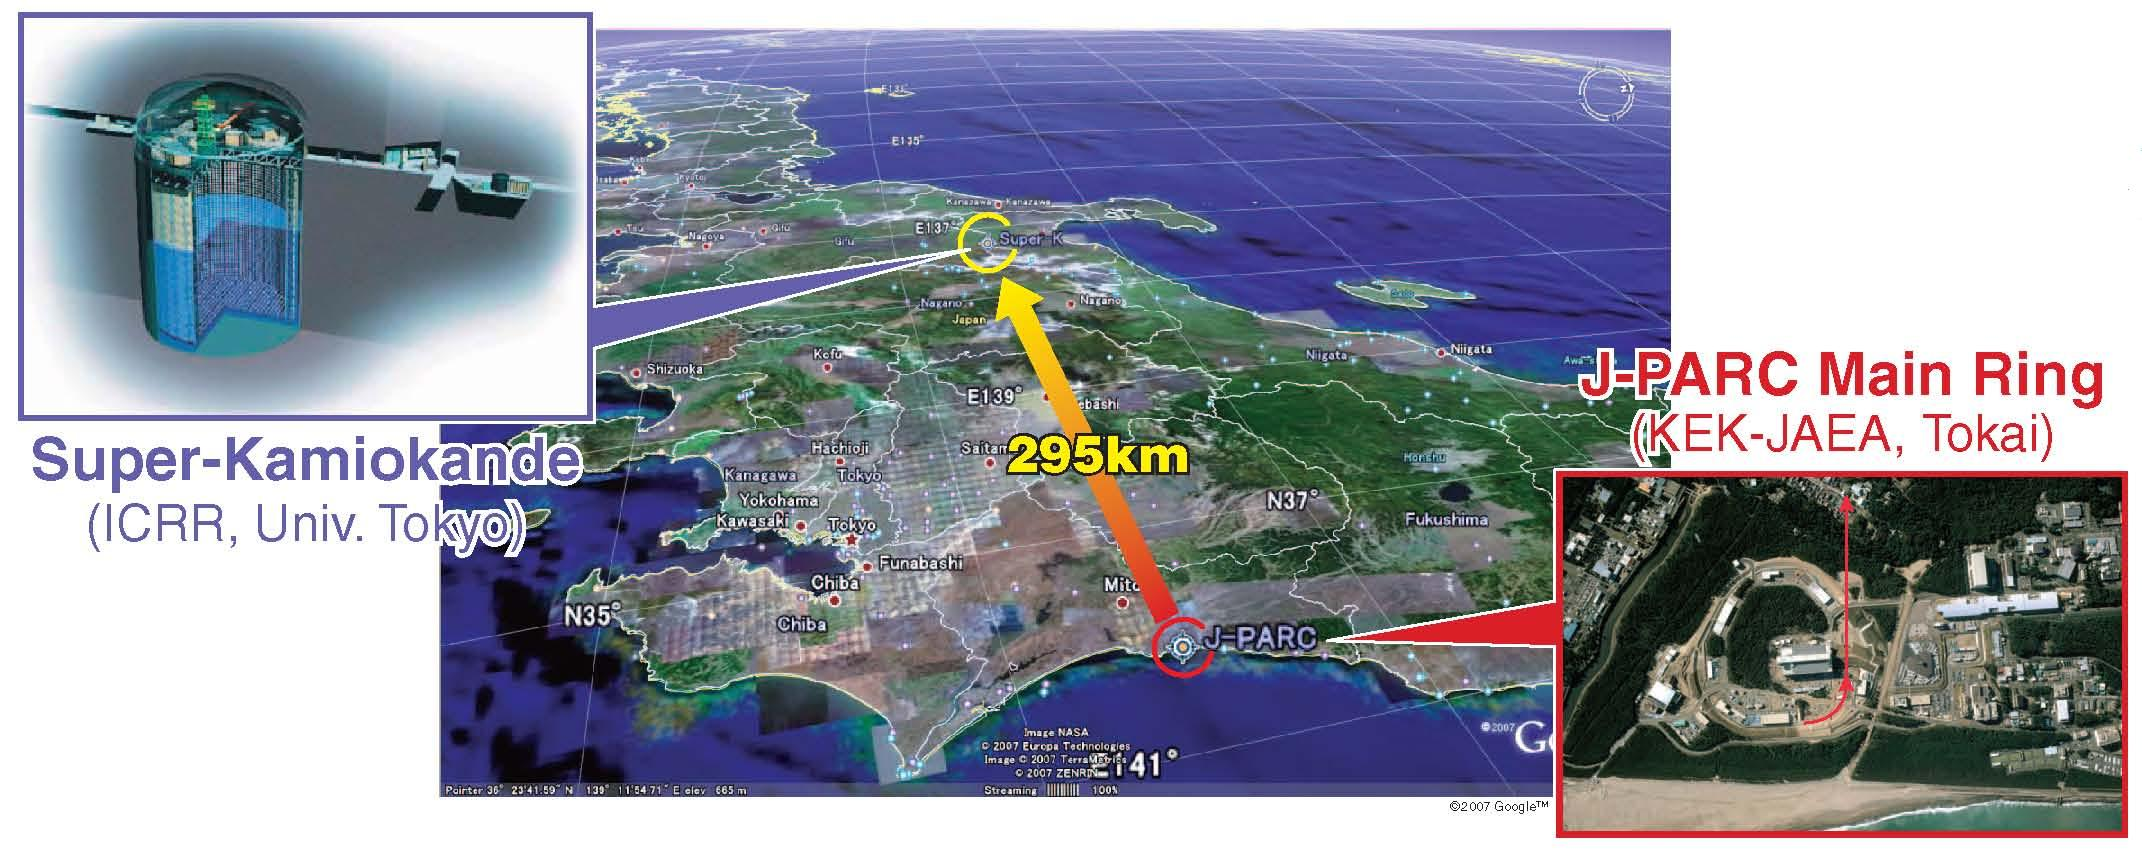
\includegraphics[width=\textwidth]{TalkPics/ComputationalPhysicsApplications/01_T2K_Birdseye-0808.jpg}
  \end{frame}

  \begin{frame}
    \frametitle{T2K}
    \begin{itemize}
    \item 463 members from 61 institutions in 11 countries
    \end{itemize}

    \centering
    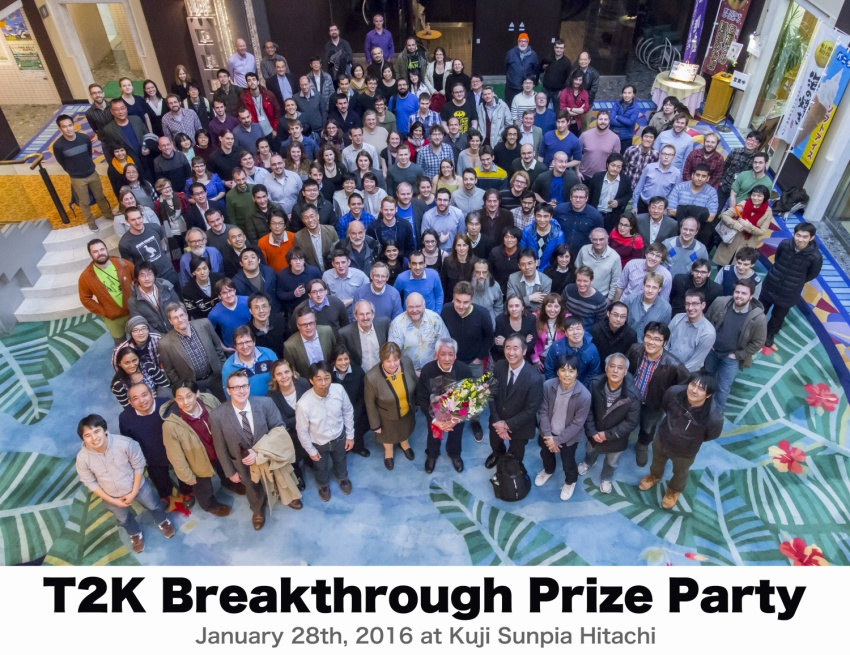
\includegraphics[width=.7\textwidth]{TalkPics/ComputationalPhysicsApplications/breakthroughparty.jpg}
  \end{frame}

  \begin{frame}
    \frametitle{T2K: ND280}
    %picture and intro
    \begin{itemize}
    \item Multi-subsystem neutrino detector 280m from beam origin
    \item Gives information about the beam before oscillation and interaction cross-section on different materials
    \end{itemize}
    \centering
    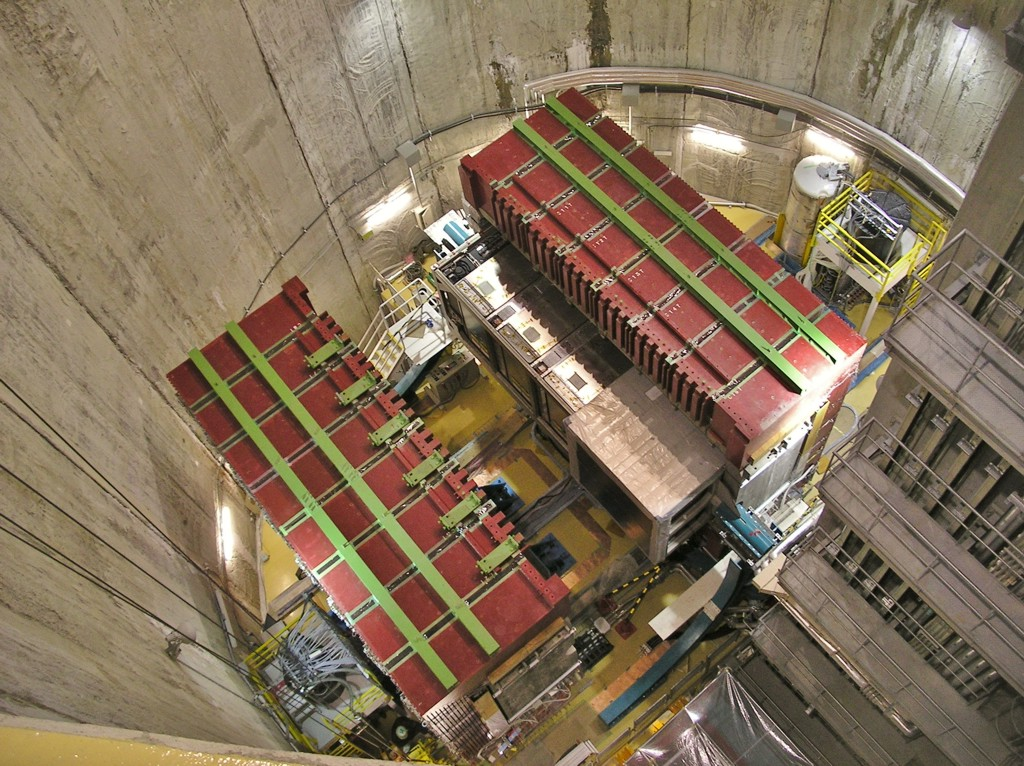
\includegraphics[height=.6\textheight]{TalkPics/ComputationalPhysicsApplications/ND280open.jpg}
    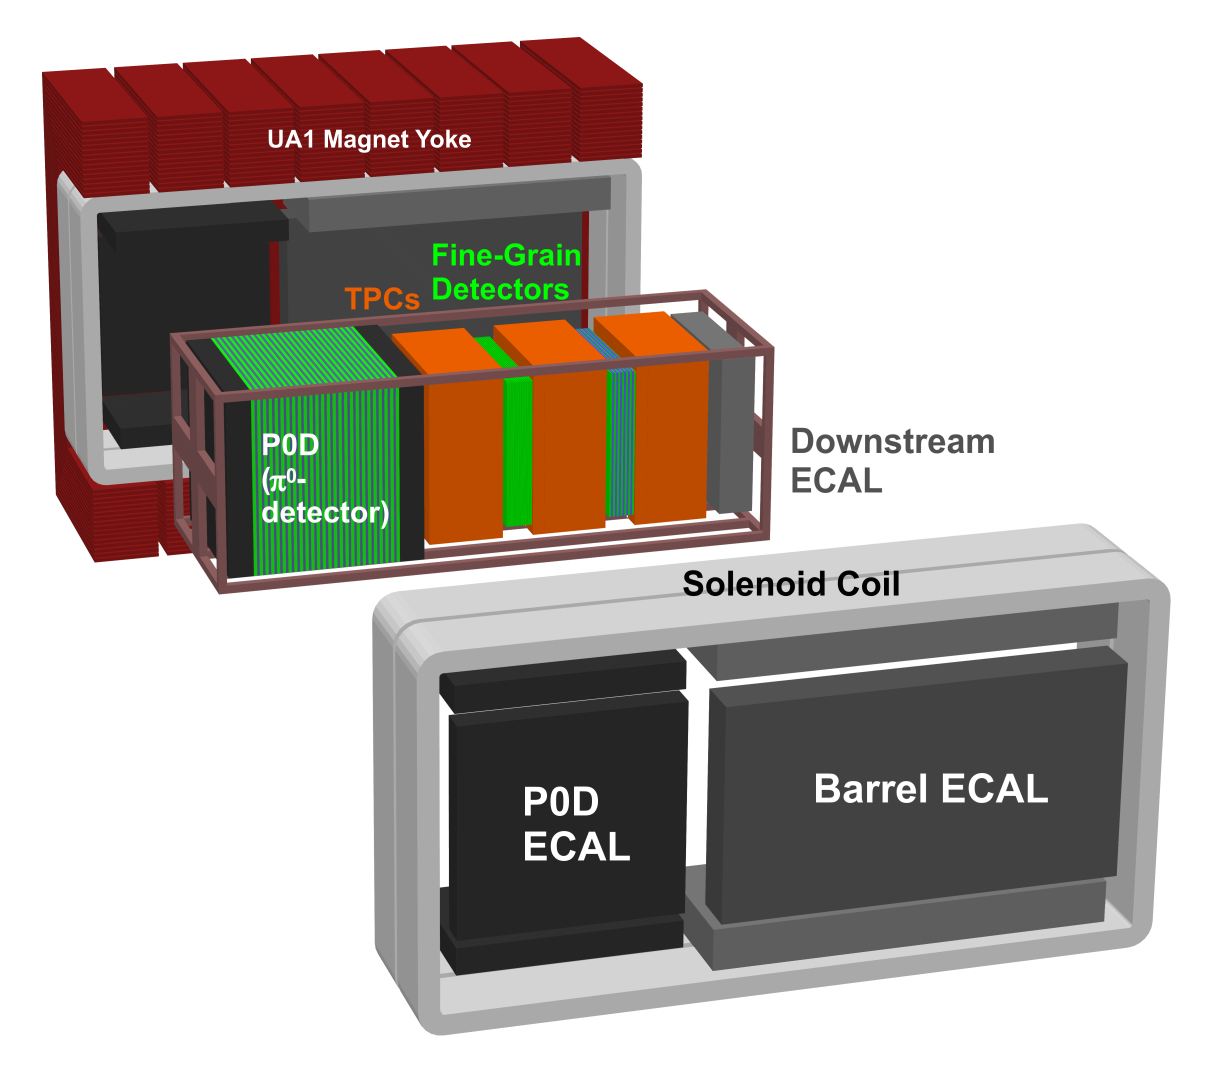
\includegraphics[height=.6\textheight]{TalkPics/ComputationalPhysicsApplications/ND280Exploded-Text-Transparent-Small.png}

  \end{frame}

  \begin{frame}
    \frametitle{T2K: SK}
    %picture and intro
    \begin{columns}
      \column{.5\textwidth}
    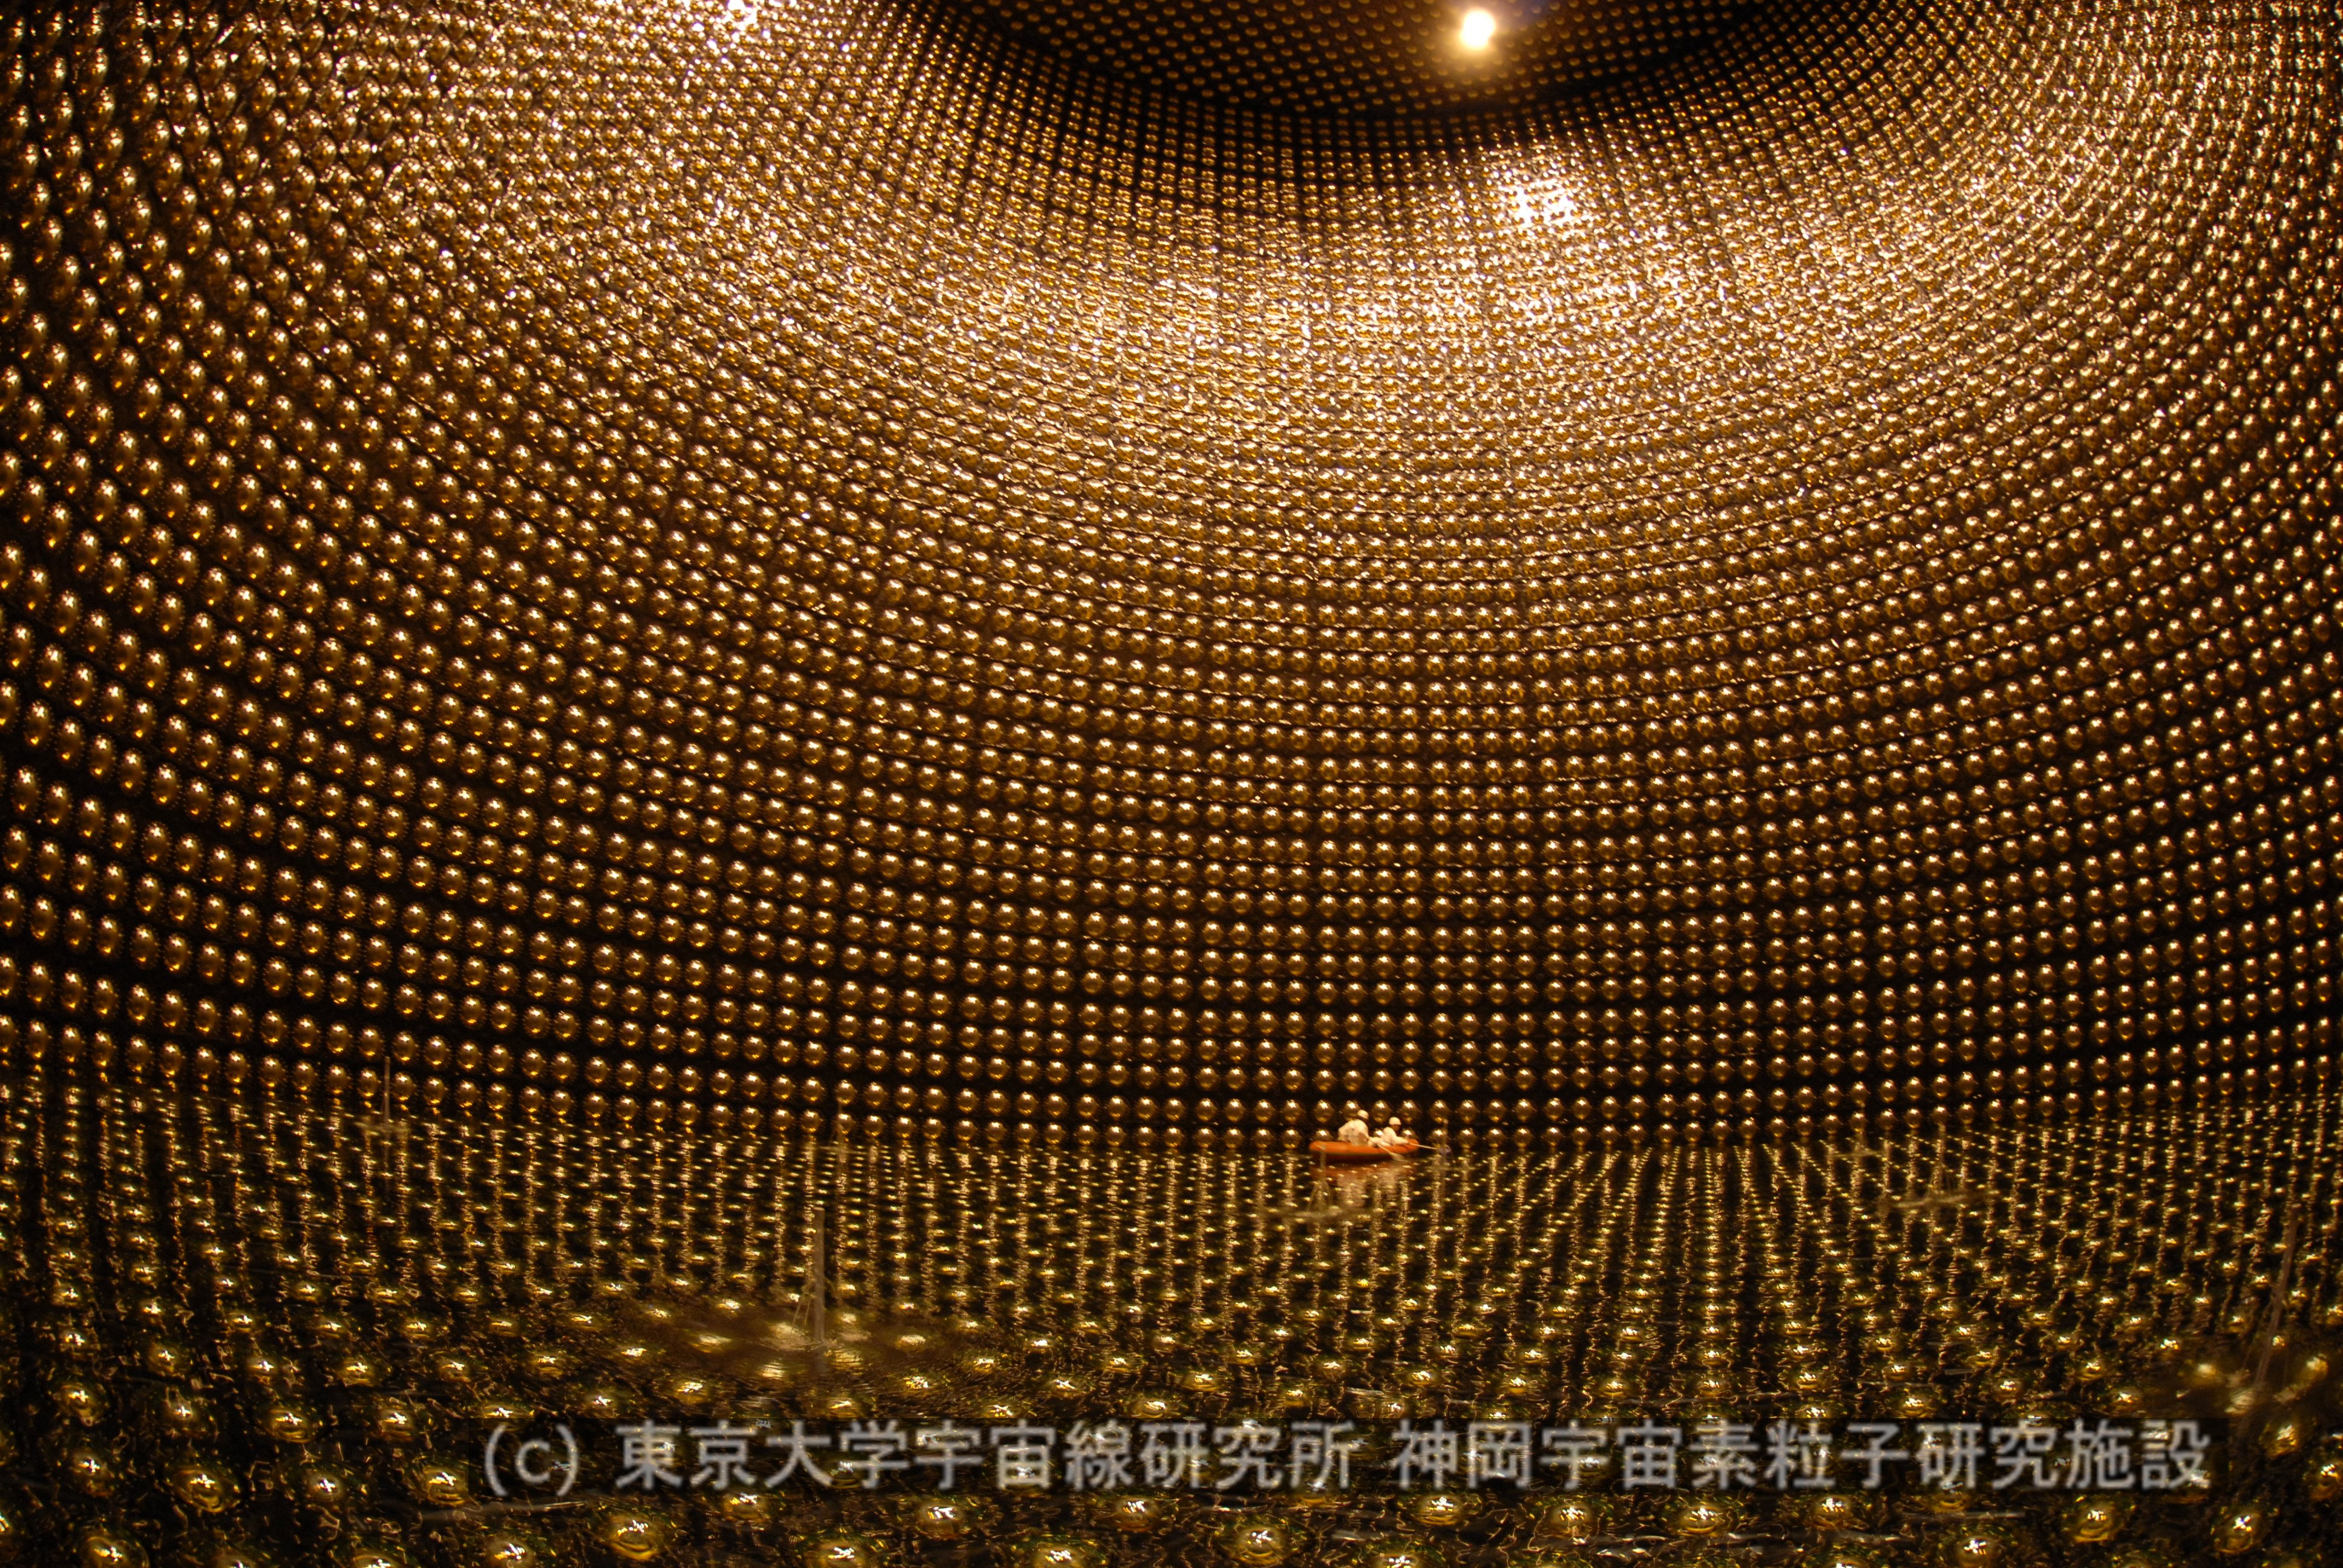
\includegraphics[width=\textwidth,height=.8\textheight]{TalkPics/ComputationalPhysicsApplications/SKinternal.jpg}
    \column{.5\textwidth}
    \begin{columns}
      \column{1.1\textwidth}
    \begin{itemize}
    \item 50kT ultra pure water
    \item 13,000 photon detectors
    \item Sees charged particles through Cherenkov light
    \item Measures the beam after oscillation
    \end{itemize}
    \end{columns}
    \vspace{.5cm}
    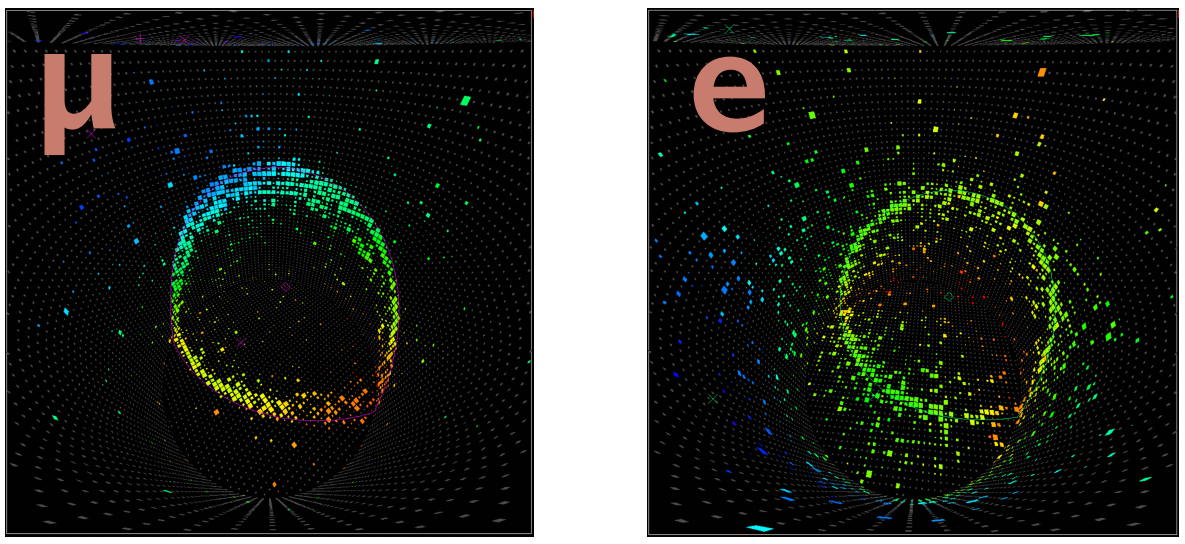
\includegraphics[width=\textwidth]{TalkPics/ComputationalPhysicsApplications/skeventdisplay.png}
    \end{columns}
  \end{frame}

  \begin{frame}
    \frametitle{How do you actually do the analysis?}
    \centering
    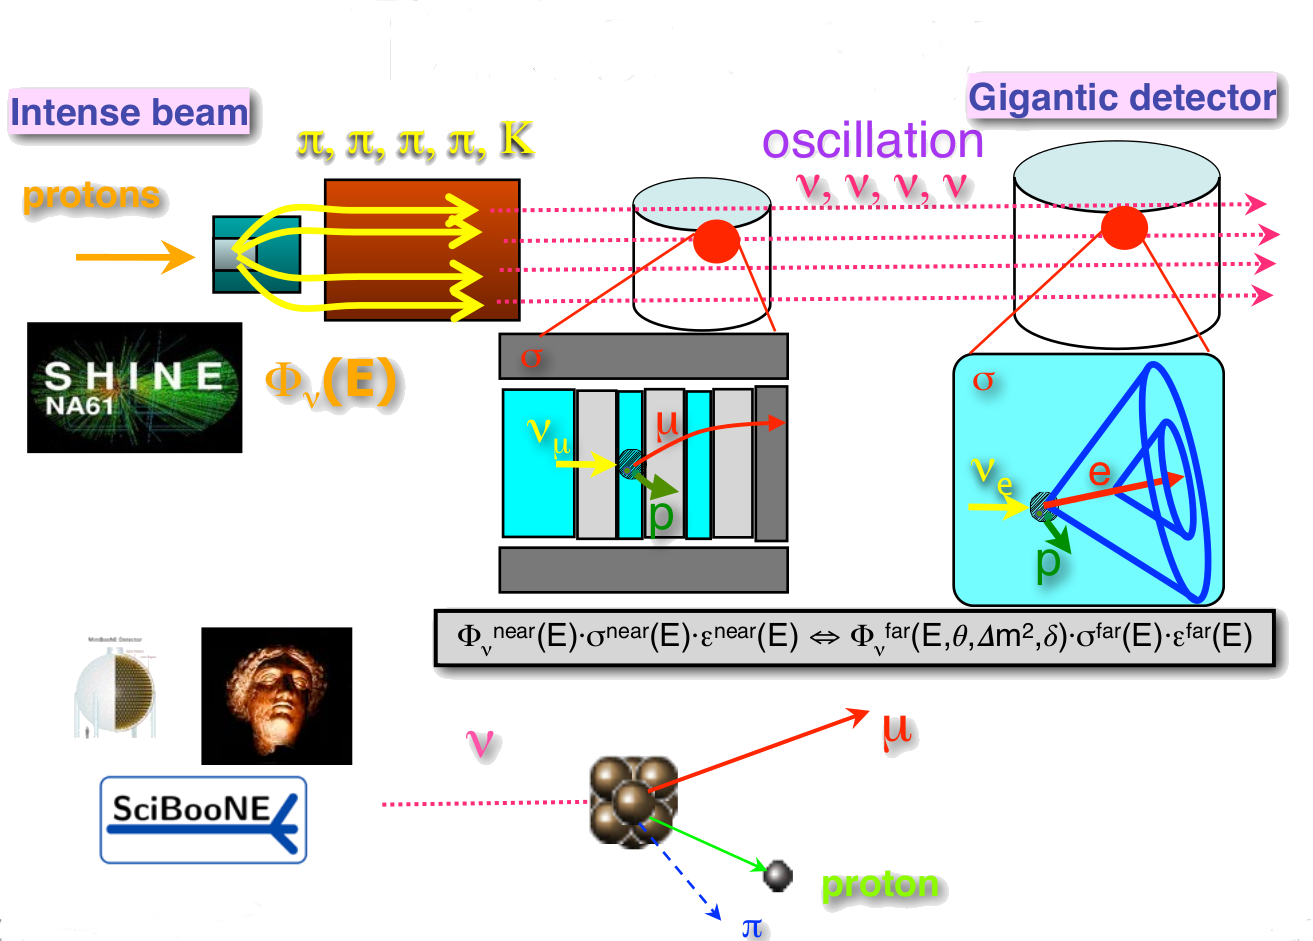
\includegraphics[width=.9\textwidth]{TalkPics/ComputationalPhysicsApplications/t2kstrategy.png}
  \end{frame}

  \begin{frame}
    \frametitle{What do we mean by complex?}
    \begin{itemize}
    \item 6 oscillation model parameters
    \item More than 700 correlated systematic parameters
    \end{itemize}
    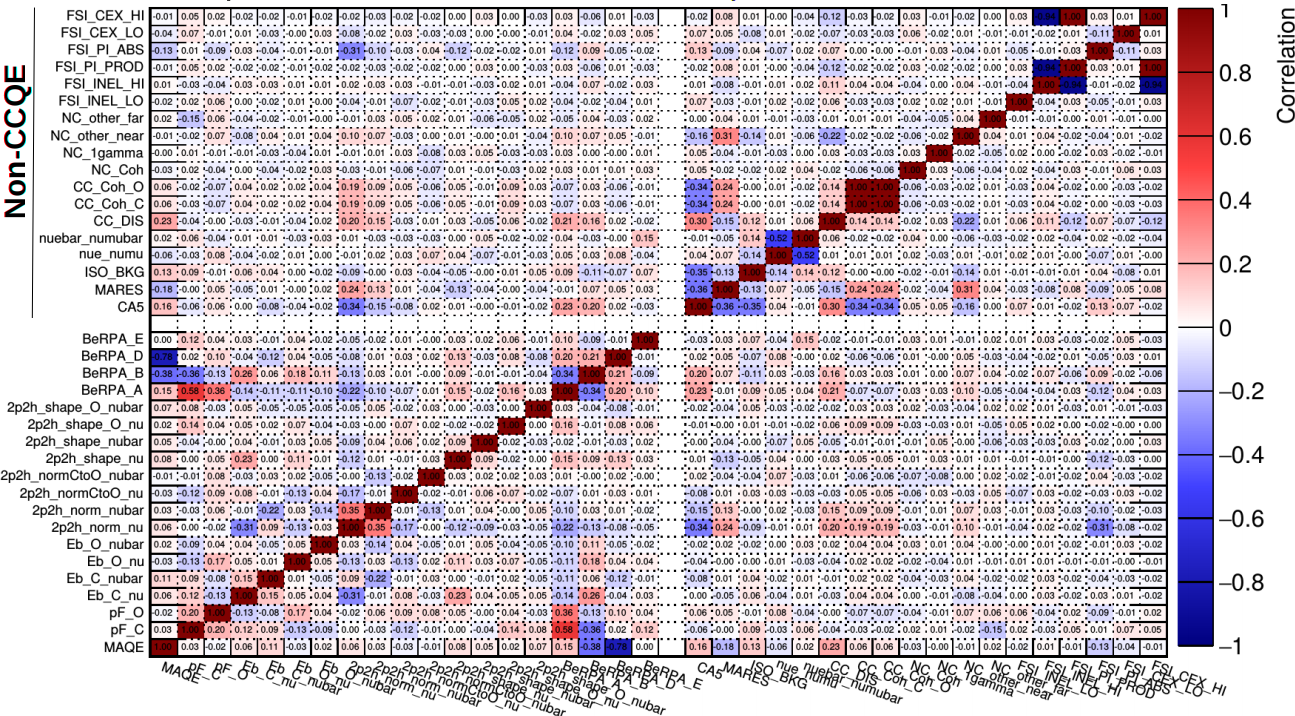
\includegraphics[width=\textwidth]{TalkPics/ComputationalPhysicsApplications/covmatrix.png}
  \end{frame}



  \begin{frame}
    \frametitle{Bayesian statistics: Posterior probability}
    \begin{itemize}
    \item Given a model can calculate probability of seeing data, D:
    \begin{equation*}
      P(D,\vec{\theta})=P(D|\vec{\theta})P(\vec{\theta})
    \end{equation*}
  \item Use Bayes theorem to turn into a statement about parameters of interest:
    \begin{equation*}
      P(\vec{\theta}|D)=\frac{P(D|\vec{\theta})P(\vec{\theta})}{\int P(D|\vec{\theta})P(\vec{\theta}\mathrm{d}\vec{\theta}}
    \end{equation*}
  \item This is a function of over 700 variables!
  \item[-] Need to eliminate all the `nuisance' parameters
  \item[-] Bayesians do this by integrating over them
    \end{itemize}
  \end{frame}

  \begin{frame}
    \frametitle{Using Monte Carlo methods}
    \begin{columns}
      \column{.5\textwidth}
      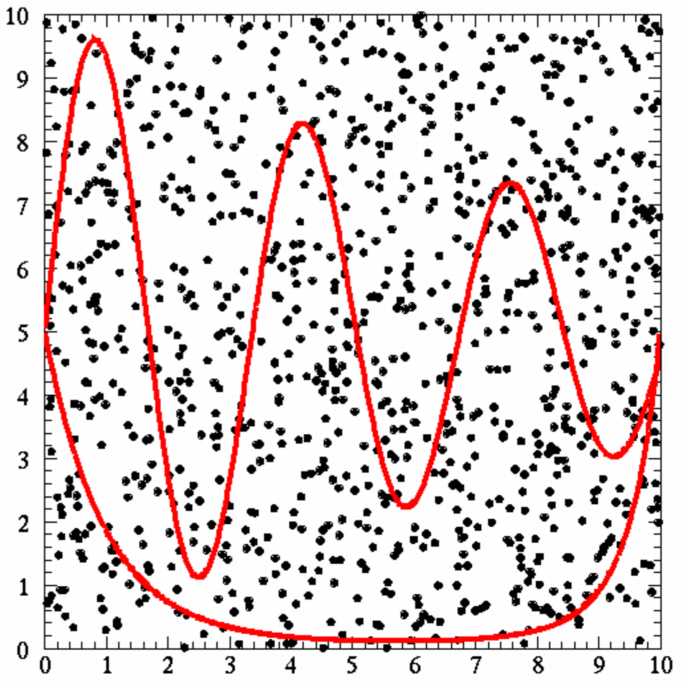
\includegraphics[width=\textwidth]{TalkPics/ComputationalPhysicsApplications/MCexample.png}
      \column{.55\textwidth}
      \begin{block}{Standard MC}
      \begin{itemize}
      \item Randomly choose points in your space
      \item Calculate the average value of your function at the points
      \item Multiply by area sampled
      \end{itemize}
      \end{block}
    \end{columns}
  \end{frame}

  \begin{frame}
    \frametitle{Using Monte Carlo methods}
    \begin{columns}
      \column{.5\textwidth}
      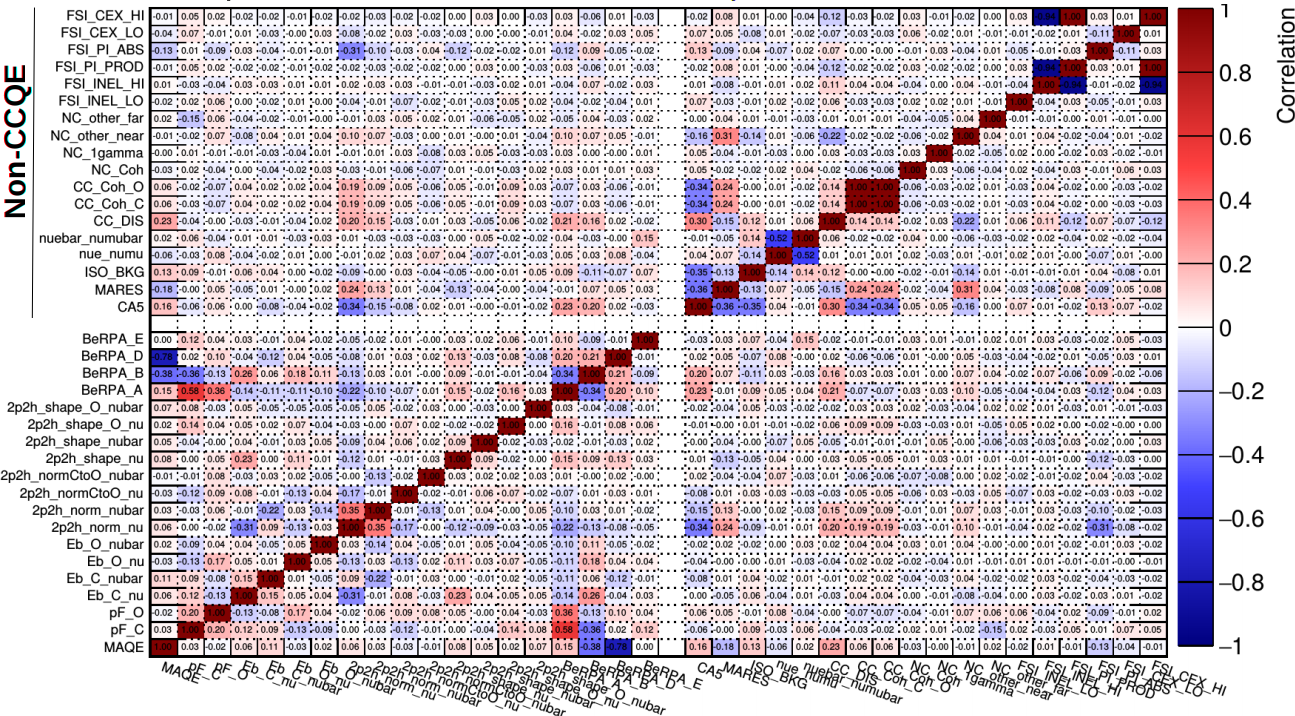
\includegraphics[width=\textwidth]{TalkPics/ComputationalPhysicsApplications/covmatrix.png}
      \column{.55\textwidth}
      \begin{block}{Problem}
        \begin{itemize}
        \item Probability is low at most points
        \item Space is very very large!
        \item[-] Over 700 dimensions
        \item Need a huge number of points
        \end{itemize}
      \end{block}
    \end{columns}
  \end{frame}





  \begin{frame}
    \frametitle{Solution: Markov Chain Monte Carlo (MCMC)}
    \begin{itemize}
    \item Need to target where the steps are thrown
      \vspace{.3cm}
    \item Use a Markov chain to 'choose' points
      \begin{itemize}
      \item[-] Next point location depends on current point
      \end{itemize}
      \vspace{.3cm}
    \item Need to avoid bias through choice of points
      \begin{itemize}
      \item[-] Make sure density of points $\propto$ probability density
      \end{itemize}
      \vspace{.3cm}
    \item How do you design a Markov chain to pick points proportional to a distribution?
    \end{itemize}
    %describe what MaCh3 tries to fit and ethos behind it
    %Metropolis MCMC from MaCh3
    %Advantages like having the full posterior
  \end{frame}

  \begin{frame}
    \frametitle{Metropolis-Hastings Algorithm}
    %describe algorithm in a few slides
    \begin{itemize}
    \item Pick a starting point $x_{0}$
    \item Calculate Probability $P(x_{0})$
    \item Don't need to know the distribution, just calculate it at a point        
    \end{itemize}
    \begin{columns}
      \column{.5\textwidth}
      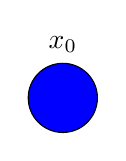
\begin{tikzpicture}
        \node[state,fill=blue,label=$x_{0}$] (A)                    {};
 %       \node[state]         (B) [above right of=A] {$q_b$};
 %       \node[state]         (D) [below right of=A] {$q_d$};
 %       \node[state]         (C) [below right of=B] {$q_c$};
 %       \node[state]         (E) [below of=D]       {$q_e$};
        %% \path (A) edge              node {0,1,L} (B)
        %%     edge              node {1,1,R} (C)
        %% (B) edge [loop above] node {1,1,L} (B)
        %%     edge              node {0,1,L} (C)
        %% (C) edge              node {0,1,L} (D)
        %%     edge [bend left]  node {1,0,R} (E)
        %% (D) edge [loop below] node {1,1,R} (D)
        %%     edge              node {0,1,R} (A)
        %% (E) edge [bend left]  node {1,0,R} (A);
      \end{tikzpicture}
      \column{.5\textwidth}
      
\includegraphics[width=\textwidth]{TalkPics/ComputationalPhysicsApplications/likelihood.png}
    \end{columns}
  \end{frame}

  \begin{frame}
    \frametitle{Metropolis-Hastings Algorithm}
    %describe algorithm in a few slides
    \begin{itemize}
    \item Propose a new point $y_{1}$ using a 'proposal function': $q(y_{1}|x_{0})$
    \item Set $x_{1}=y_{1}$ with probability:
      \begin{equation*}
        \alpha=min\left(1,\frac{P(y_{1})q(y_{1}|x_{0})}{P(x_{0})q(x_{0}|y_{1})}\right)
      \end{equation*}
    \end{itemize}
    \begin{columns}
      \column{.5\textwidth}
      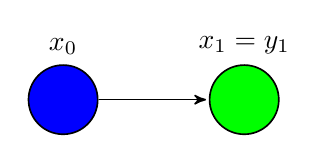
\begin{tikzpicture}[->,>=stealth',shorten >=1pt,auto,node distance=2.3cm,
                    semithick]
        \node[state,fill=blue,label=$x_{0}$] (A)                    {};
        \node[state,fill=green,label={$x_{1}=y_{1}$}] (B)       [right of=A,] {};
 %       \node[state]         (D) [below right of=A] {$q_d$};
 %       \node[state]         (C) [below right of=B] {$q_c$};
 %       \node[state]         (E) [below of=D]       {$q_e$};
        \path (A) edge []             node {} (B);
        %%     edge              node {1,1,R} (C)
        %%(A) edge [loop above,dashed] node {reject} (A);
        %%     edge              node {0,1,L} (C)
        %% (C) edge              node {0,1,L} (D)
        %%     edge [bend left]  node {1,0,R} (E)
        %% (D) edge [loop below] node {1,1,R} (D)
        %%     edge              node {0,1,R} (A)
        %% (E) edge [bend left]  node {1,0,R} (A);
      \end{tikzpicture}

      \column{.5\textwidth}
      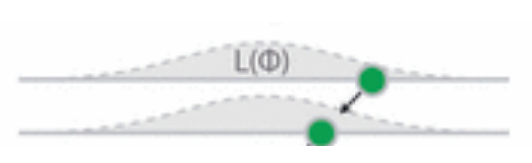
\includegraphics[width=\textwidth]{TalkPics/ComputationalPhysicsApplications/likelihoodstep.png}
    \end{columns}
  \end{frame}


  \begin{frame}
    \frametitle{Metropolis-Hastings Algorithm}
    \begin{columns}
      \column{.5\textwidth}
      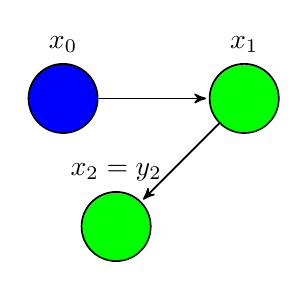
\begin{tikzpicture}[->,>=stealth',shorten >=1pt,auto,node distance=2.3cm,
                    semithick]
        \node[state,fill=blue,label=$x_{0}$] (A)                    {};
        \node[state,fill=green,label=$x_{1}$] (B)       [right of=A,] {};
        \node[state,fill=green,label={$x_{2}=y_{2}$}] (C)       [below left of=B,] {};
 %       \node[state]         (D) [below right of=A] {$q_d$};
 %       \node[state]         (C) [below right of=B] {$q_c$};
 %       \node[state]         (E) [below of=D]       {$q_e$};
        \path (A) edge []             node {} (B)
        (B) edge []             node {} (C);
        %%     edge              node {1,1,R} (C)
        %%(A) edge [loop above,dashed] node {reject} (A);
        %%     edge              node {0,1,L} (C)
        %% (C) edge              node {0,1,L} (D)
        %%     edge [bend left]  node {1,0,R} (E)
        %% (D) edge [loop below] node {1,1,R} (D)
        %%     edge              node {0,1,R} (A)
        %% (E) edge [bend left]  node {1,0,R} (A);
      \end{tikzpicture}
      \column{.5\textwidth}
      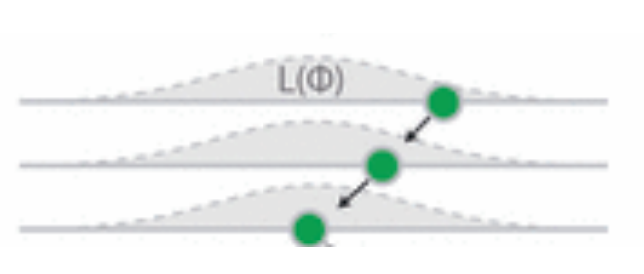
\includegraphics[width=\textwidth]{TalkPics/ComputationalPhysicsApplications/likelihoodstep2.png}
      \end{columns}
  \end{frame}


  \begin{frame}
    \frametitle{Metropolis-Hastings Algorithm}
    \begin{columns}
      \column{.5\textwidth}
      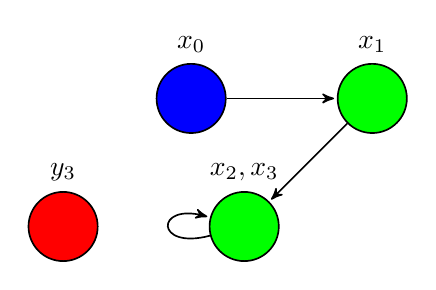
\begin{tikzpicture}[->,>=stealth',shorten >=1pt,auto,node distance=2.3cm,
                    semithick]
        \node[state,fill=blue,label=$x_{0}$] (A)                    {};
        \node[state,fill=green,label=$x_{1}$] (B)       [right of=A,] {};
        \node[state,fill=green,label={$x_{2},x_{3}$}] (C)       [below left of=B,] {};
        \node[state,fill=red,label=$y_{3}$] (D)       [left of=C,] {};
 %       \node[state]         (D) [below right of=A] {$q_d$};
 %       \node[state]         (C) [below right of=B] {$q_c$};
 %       \node[state]         (E) [below of=D]       {$q_e$};
        \path (A) edge []             node {} (B)
        (B) edge []             node {} (C)
        (C) edge [loop left]             node {} (C);
        %%     edge              node {1,1,R} (C)
        %%(A) edge [loop above,dashed] node {reject} (A);
        %%     edge              node {0,1,L} (C)
        %% (C) edge              node {0,1,L} (D)
        %%     edge [bend left]  node {1,0,R} (E)
        %% (D) edge [loop below] node {1,1,R} (D)
        %%     edge              node {0,1,R} (A)
        %% (E) edge [bend left]  node {1,0,R} (A);
      \end{tikzpicture}
      \column{.5\textwidth}
      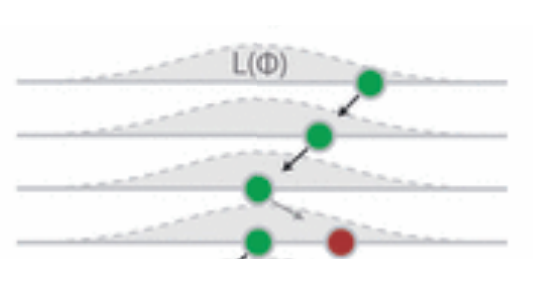
\includegraphics[width=\textwidth]{TalkPics/ComputationalPhysicsApplications/likelihoodstep3.png}
      \end{columns}
    \vspace{.3cm}
    \begin{itemize}
    \item $P(y_{3})<P(x_{2})$ so $\alpha<1$ and it might be rejected
    \end{itemize}
  \end{frame}


  \begin{frame}
    \frametitle{Metropolis-Hastings Algorithm}
    \begin{columns}
      \column{.5\textwidth}
      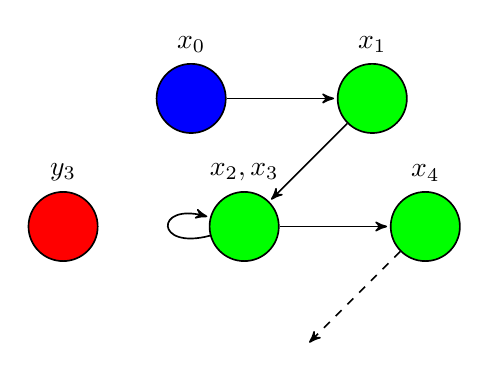
\begin{tikzpicture}[->,>=stealth',shorten >=1pt,auto,node distance=2.3cm,
                    semithick]
        \node[state,fill=blue,label=$x_{0}$] (A)                    {};
        \node[state,fill=green,label=$x_{1}$] (B)       [right of=A,] {};
        \node[state,fill=green,label={$x_{2},x_{3}$}] (C)       [below left of=B,] {};
        \node[state,fill=red,label=$y_{3}$] (D)       [left of=C,] {};
        \node[state,fill=green,label=$x_{4}$] (E)       [right of=C,] {};
        \node[] (F)       [below left of=E,] {};
 %       \node[state]         (D) [below right of=A] {$q_d$};
 %       \node[state]         (C) [below right of=B] {$q_c$};
 %       \node[state]         (E) [below of=D]       {$q_e$};
        \path (A) edge []             node {} (B)
        (B) edge []             node {} (C)
        (C) edge [loop left]             node {} (C)
        (C) edge []             node {} (E)
        (E) edge [dashed]             node {} (F);

        %%     edge              node {1,1,R} (C)
        %%(A) edge [loop above,dashed] node {reject} (A);
        %%     edge              node {0,1,L} (C)
        %% (C) edge              node {0,1,L} (D)
        %%     edge [bend left]  node {1,0,R} (E)
        %% (D) edge [loop below] node {1,1,R} (D)
        %%     edge              node {0,1,R} (A)
        %% (E) edge [bend left]  node {1,0,R} (A);
      \end{tikzpicture}

      \begin{itemize}
      \item Repeat until you build up a picture of the probability
      \end{itemize}
      \column{.5\textwidth}
      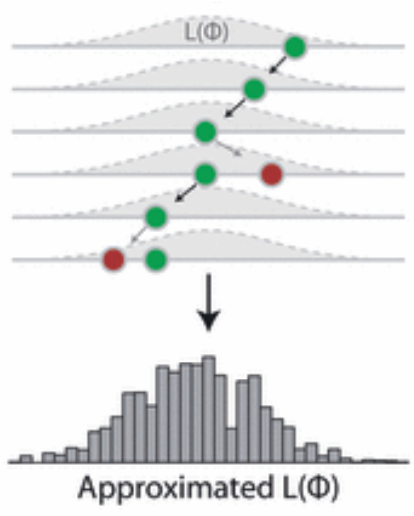
\includegraphics[width=\textwidth]{TalkPics/ComputationalPhysicsApplications/likelihoodstep4.png}
      \end{columns}
  \end{frame}

  \begin{frame}
    \frametitle{How do we know the MCMC is representative?}
    \begin{itemize}
    \item There are three conditions for a Markov Chain to converge to being representative of a distribution:
      \begin{itemize}
      \item[1] Irreducibility: Must be possible to get from one point to any other point in a finite number of steps
      \item[2] Recurrence: Each step after convergence must be a sample from the distribution
      \item[3] Aperiodicity: The chain must not move periodically through the same sequence of states
      \end{itemize}
    \item Need to choose the right proposal function and acceptance probability
    \end{itemize}
  \end{frame}

  \begin{frame}
    \frametitle{Which Proposal Function do we use?}
    \begin{columns}
      \column{.5\textwidth}
      \begin{block}{Continuous parameter}
        \begin{itemize}
        \item Use a multivariate Gaussian
        \item Take into account correlation between parameters
        \item Satisfies irreducibility \checkmark
        \item Satisfies aperiodicity \checkmark
        \end{itemize}
      \end{block}
      %Gaussian for continuous parameters, 50% chance of flip for discrete
      %point out symmetrical in our case
      \column{.5\textwidth}
      \begin{block}{Discrete parameter}
        \begin{itemize}
        \item All discrete parameters we look at have 2 values
        \item 50\% chance of flipping for any step
        \item Satisfies irreducibility \checkmark 
        \item Satisfies aperiodicity \checkmark
        \end{itemize}
      \end{block}
    \end{columns}
    
    \begin{itemize}
    \item Both of these are symmetrical so:
    \item[-] $\rightarrow \alpha=min\left(1,\frac{P(y_{1})}{P(x_{0})}\right)$
    \item Each step is therefore a sample from P
    \item[-] Satisfies recurrence \checkmark
    \end{itemize}

  \end{frame}

  \begin{frame}
    \frametitle{Which Proposal Function?}
    \begin{itemize}
    \item Need to pick a width for the Gaussian
    \item Too wide and a lot of steps will be rejected:
      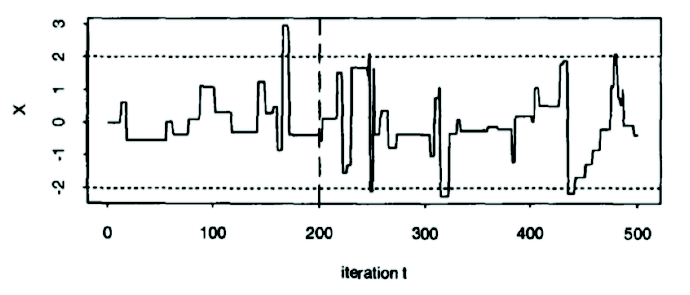
\includegraphics[height=.2\textheight,width=.7\textwidth]{TalkPics/ComputationalPhysicsApplications/toobigstep.png}
    \item Too narrow takes too long to 'forget' initial conditions:
      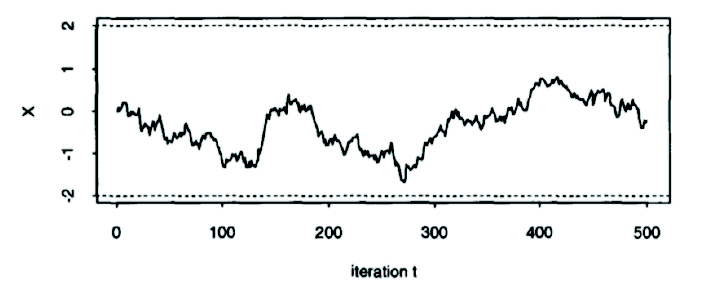
\includegraphics[height=.2\textheight,width=.7\textwidth]{TalkPics/ComputationalPhysicsApplications/toosmallstep.png}
    \item Just right and it explores space and converges quickly:
      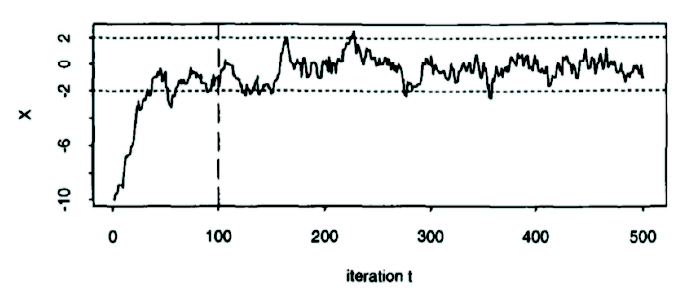
\includegraphics[height=.2\textheight,width=.7\textwidth]{TalkPics/ComputationalPhysicsApplications/justrightstep.png}
    \end{itemize}
    %Example of some step sizes
  \end{frame}

  \begin{frame}
    \frametitle{MCMC: Burn In}
    \begin{itemize}
    \item Initial period not representative of distribution
    \item We cut off the first 20k steps of the chain
    \end{itemize}
    %Example of burn in
    \centering
    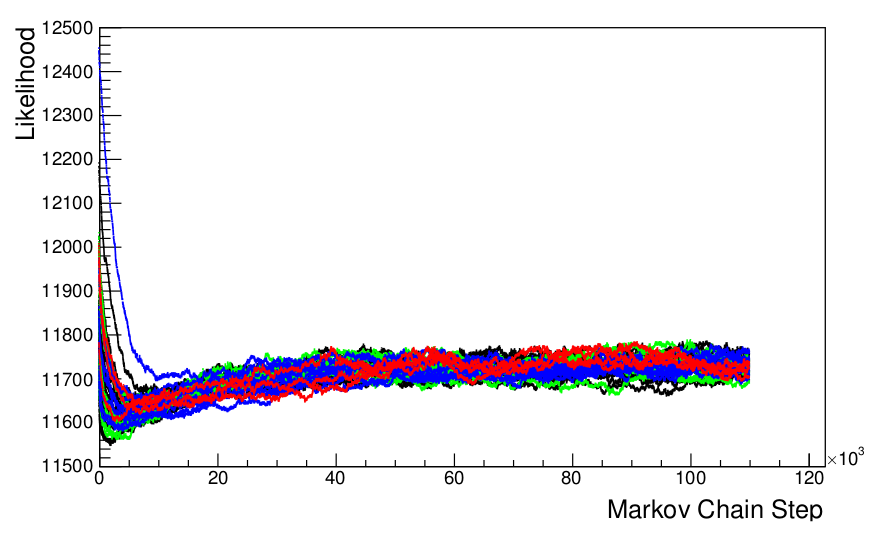
\includegraphics[width=.85\textwidth]{TalkPics/ComputationalPhysicsApplications/likelihoodvsstep.png}
  \end{frame}

  \begin{frame}
    \frametitle{Implementation}
    \begin{columns}
      \column{1.1\textwidth}
    \begin{itemize}
    \item Representative chain needs several million steps
    \item Takes $\sim$24 hours using multiple machines and GPU acceleration
    \item Code written in C++ and CUDA (GPU langauge)
      \begin{itemize}
      \item We have 8 active developers
      \item s/step $\sim$0.5 with GPU, $\sim$2.5 without GPU
      \end{itemize}
    \end{itemize}
    \end{columns}

    \centering

    \hfill
    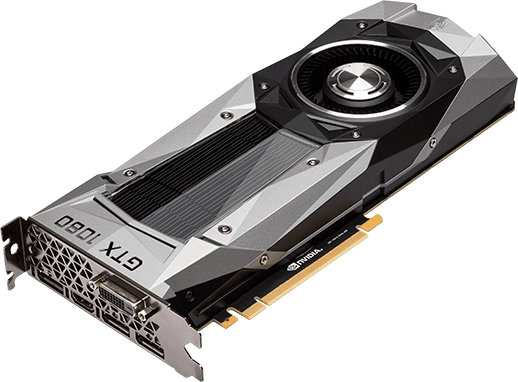
\includegraphics[height=.5\textheight]{TalkPics/ComputationalPhysicsApplications/gpupic.png}
    \hfill
    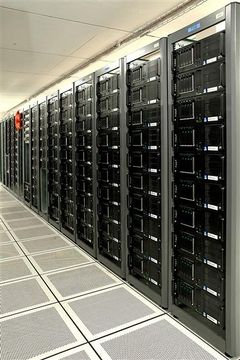
\includegraphics[height=.5\textheight]{../invisible/TalkPics/sgs120315/HLT.jpg}
    \hfill
  \end{frame}

\begin{frame}
    \frametitle{MCMC: Results}
    %??Some results
    \begin{itemize}
    \item Draw contours around regions containing 68/90\% of all steps
    \item Region inside/outside contour is 'allowed'/'excluded'
    \end{itemize}
    \centering
    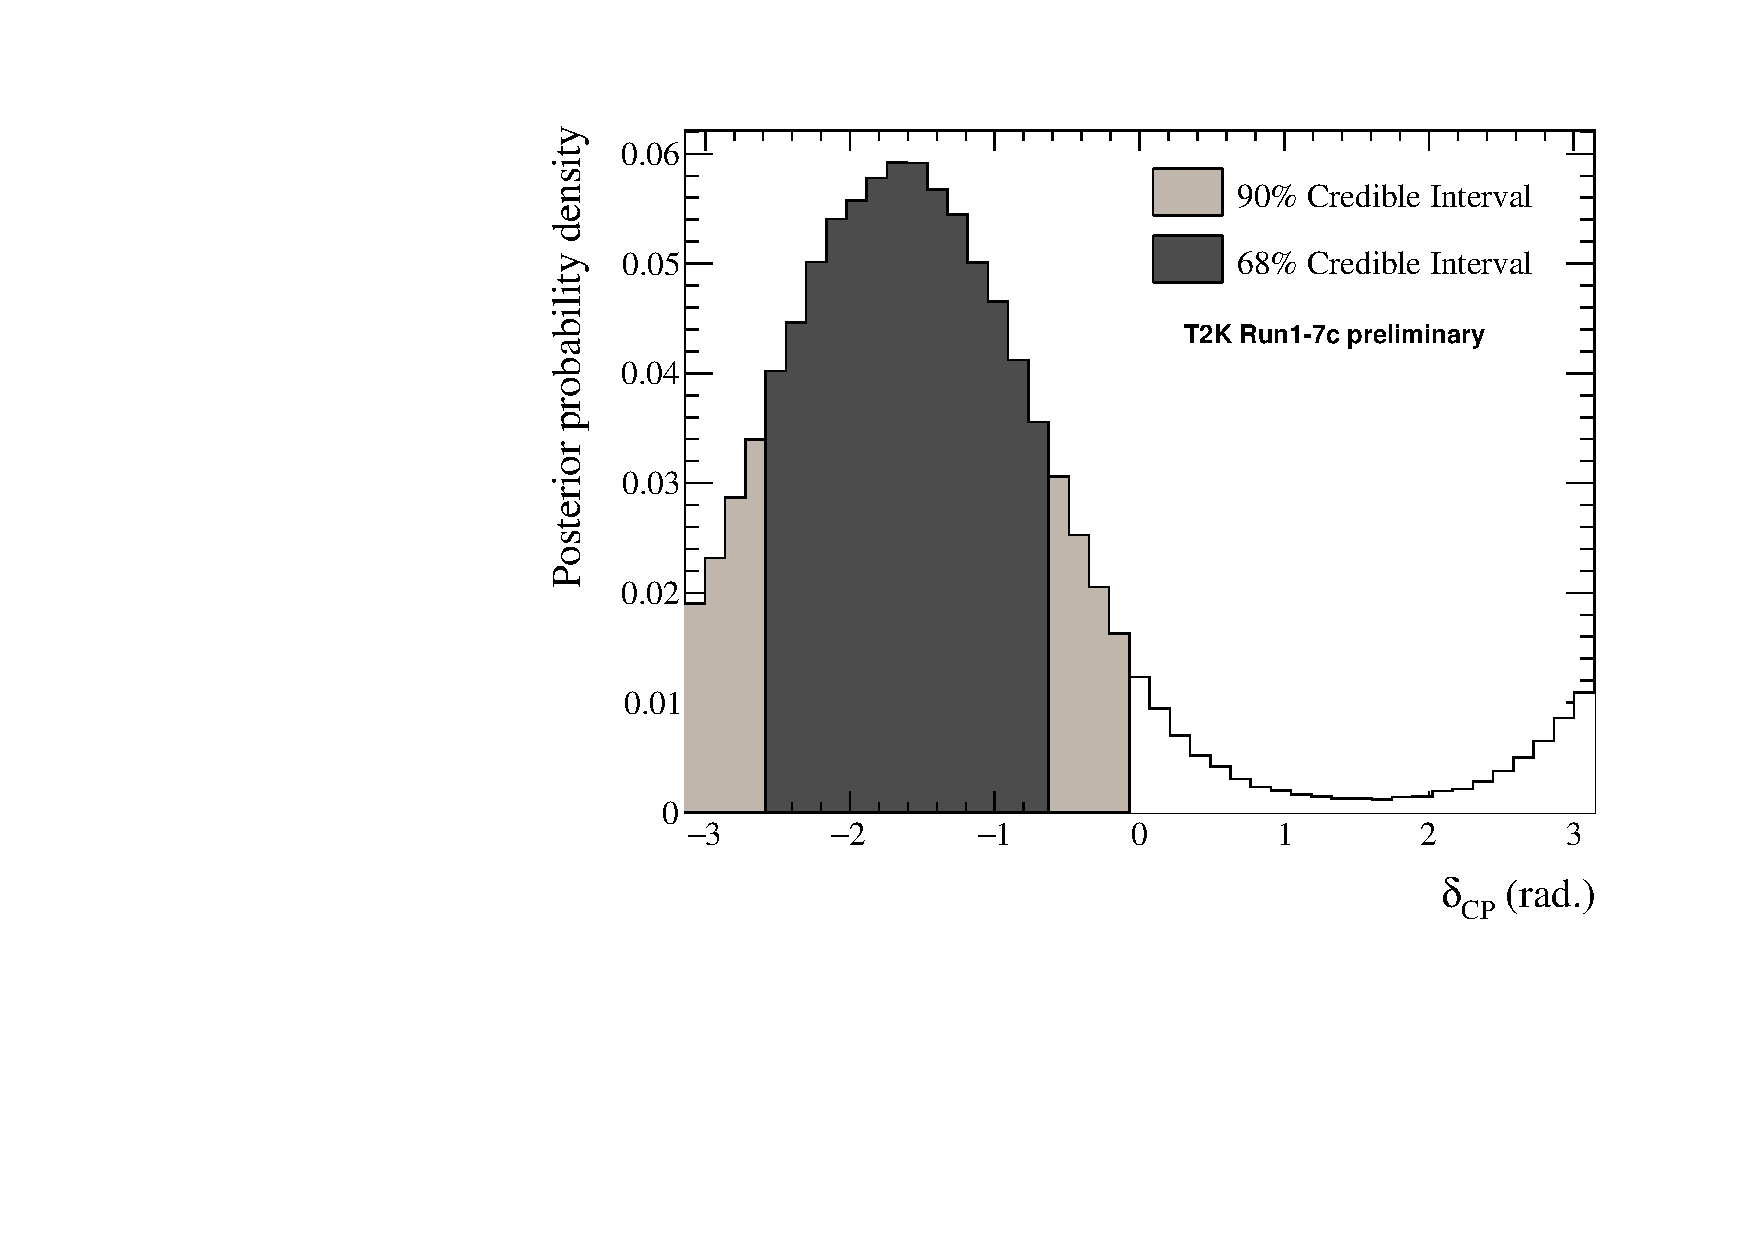
\includegraphics[height=.5\textheight]{TalkPics/ComputationalPhysicsApplications/mach3dcp.pdf}
    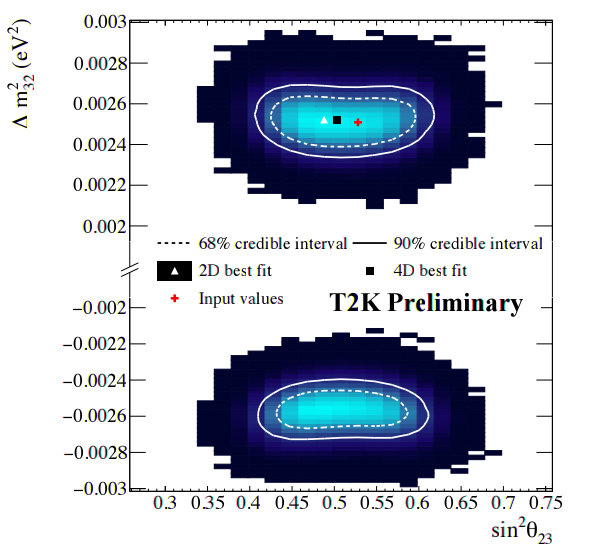
\includegraphics[height=.5\textheight]{TalkPics/ComputationalPhysicsApplications/mach3disapp.png}
 \end{frame}
  
  
  
  \begin{frame}
    \frametitle{Validation}
    \begin{itemize}
    \item Highly complex code and inputs so validation necessary
    \item T2K has two other oscillation fitters
    \item Validate results from all three fitters against each other
    \end{itemize}
    %??how long we spend validating against other analyses
    %?? mach3, ptheta, valor plots
    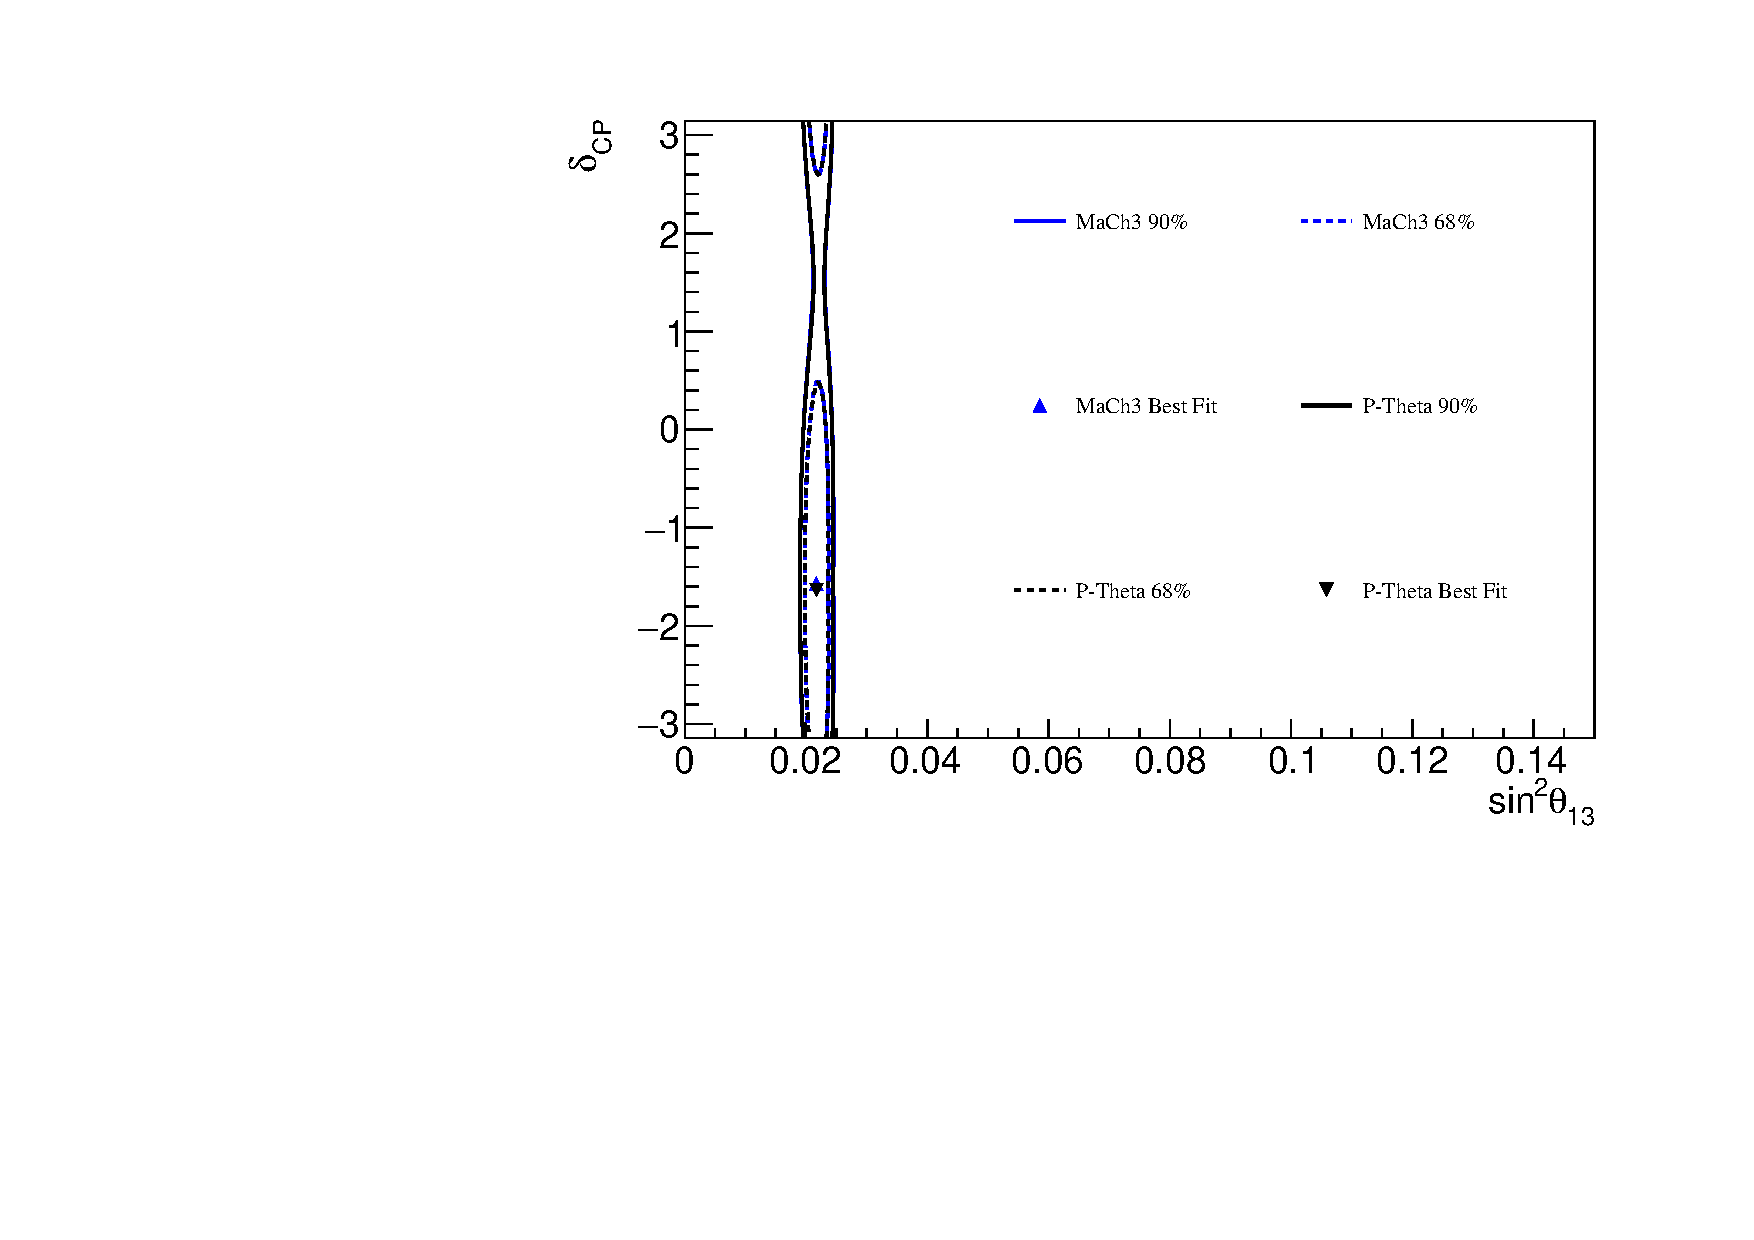
\includegraphics[width=.55\textwidth]{TalkPics/ComputationalPhysicsApplications/comparedcontours_2D_threeanalyses_wRC_th13dcp_NH.pdf}
    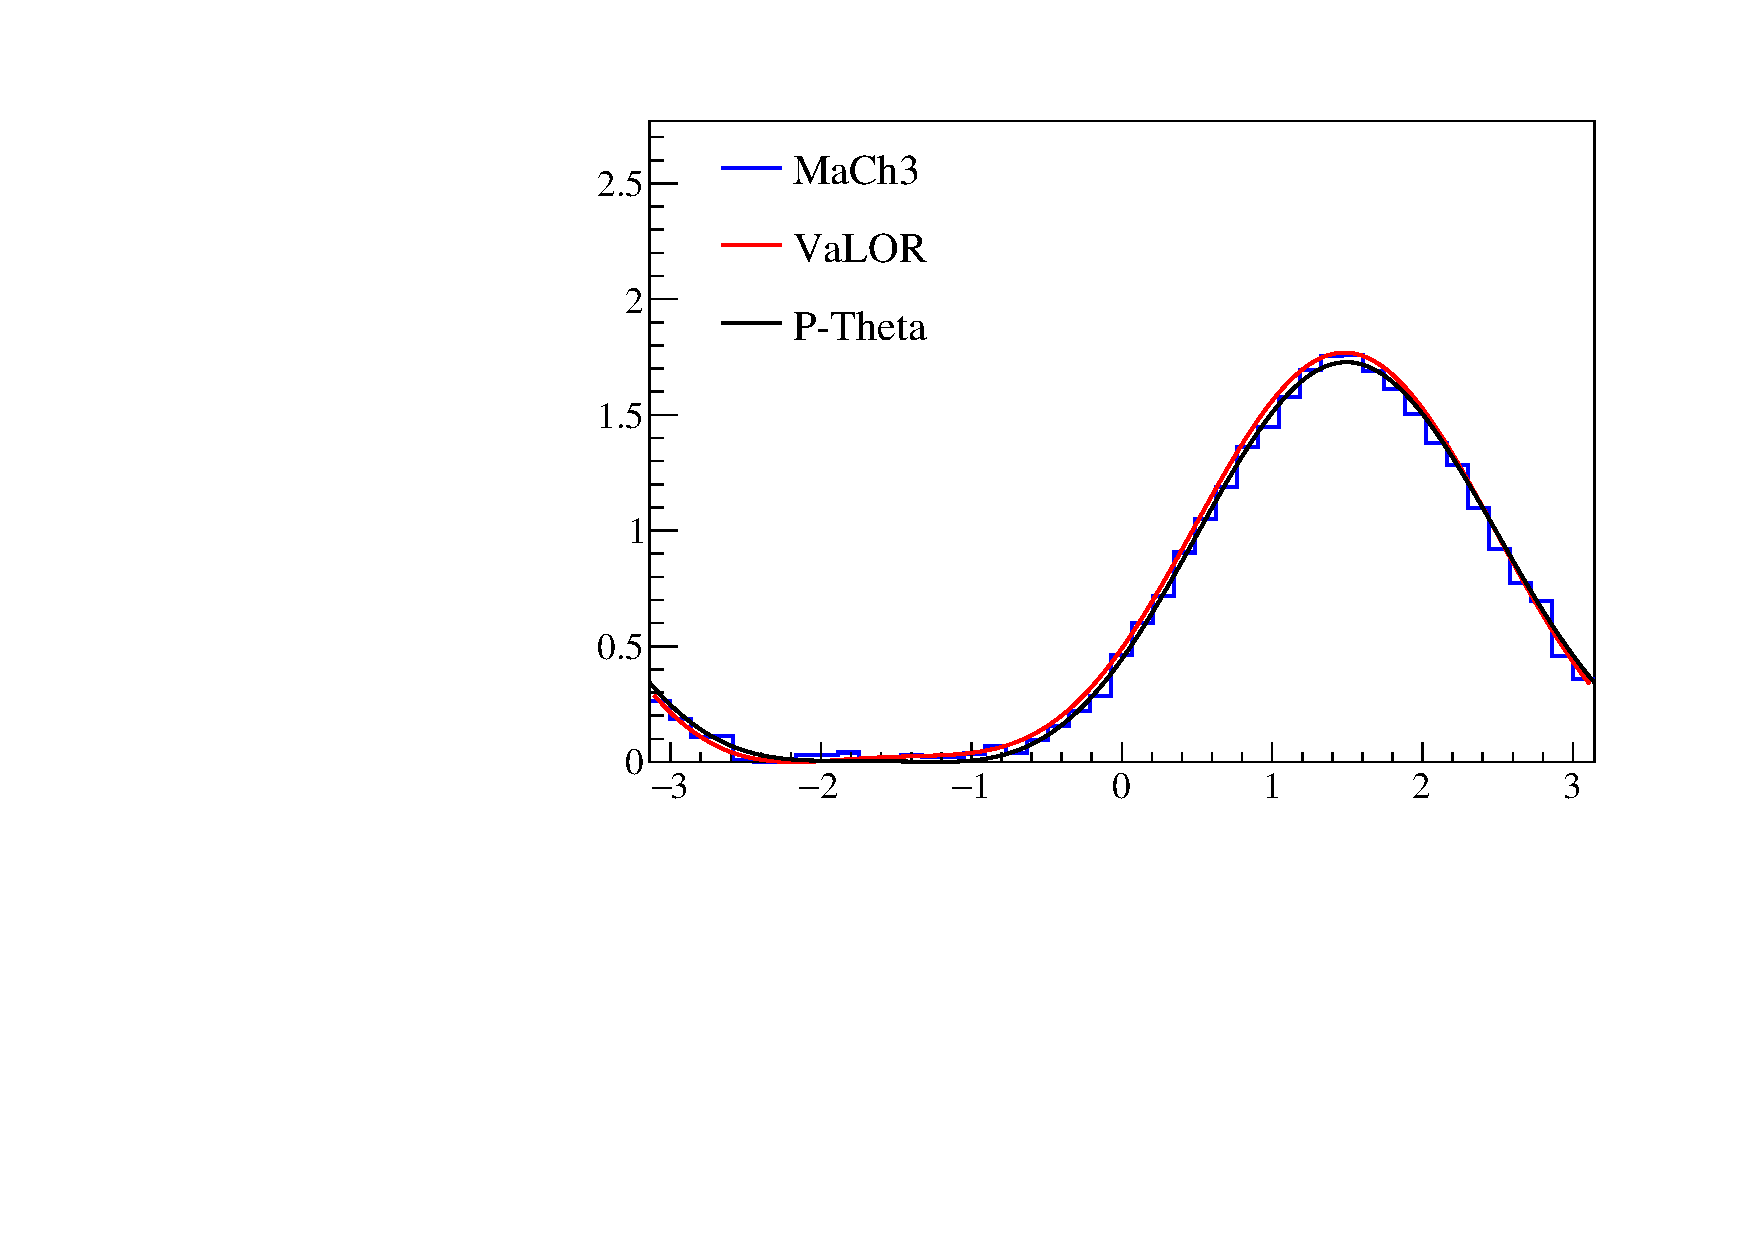
\includegraphics[width=.55\textwidth]{TalkPics/ComputationalPhysicsApplications/comparedcontours_2D_threeanalyses_woRC_dcp_NH.pdf}
  \end{frame}

  \begin{frame}
    \frametitle{The Large Hadron Collider (LHC)}
    \begin{itemize}
    \item LHC in Geneva is a 27km long, 14 TeV proton synchrotron
    \end{itemize}
    \centering
    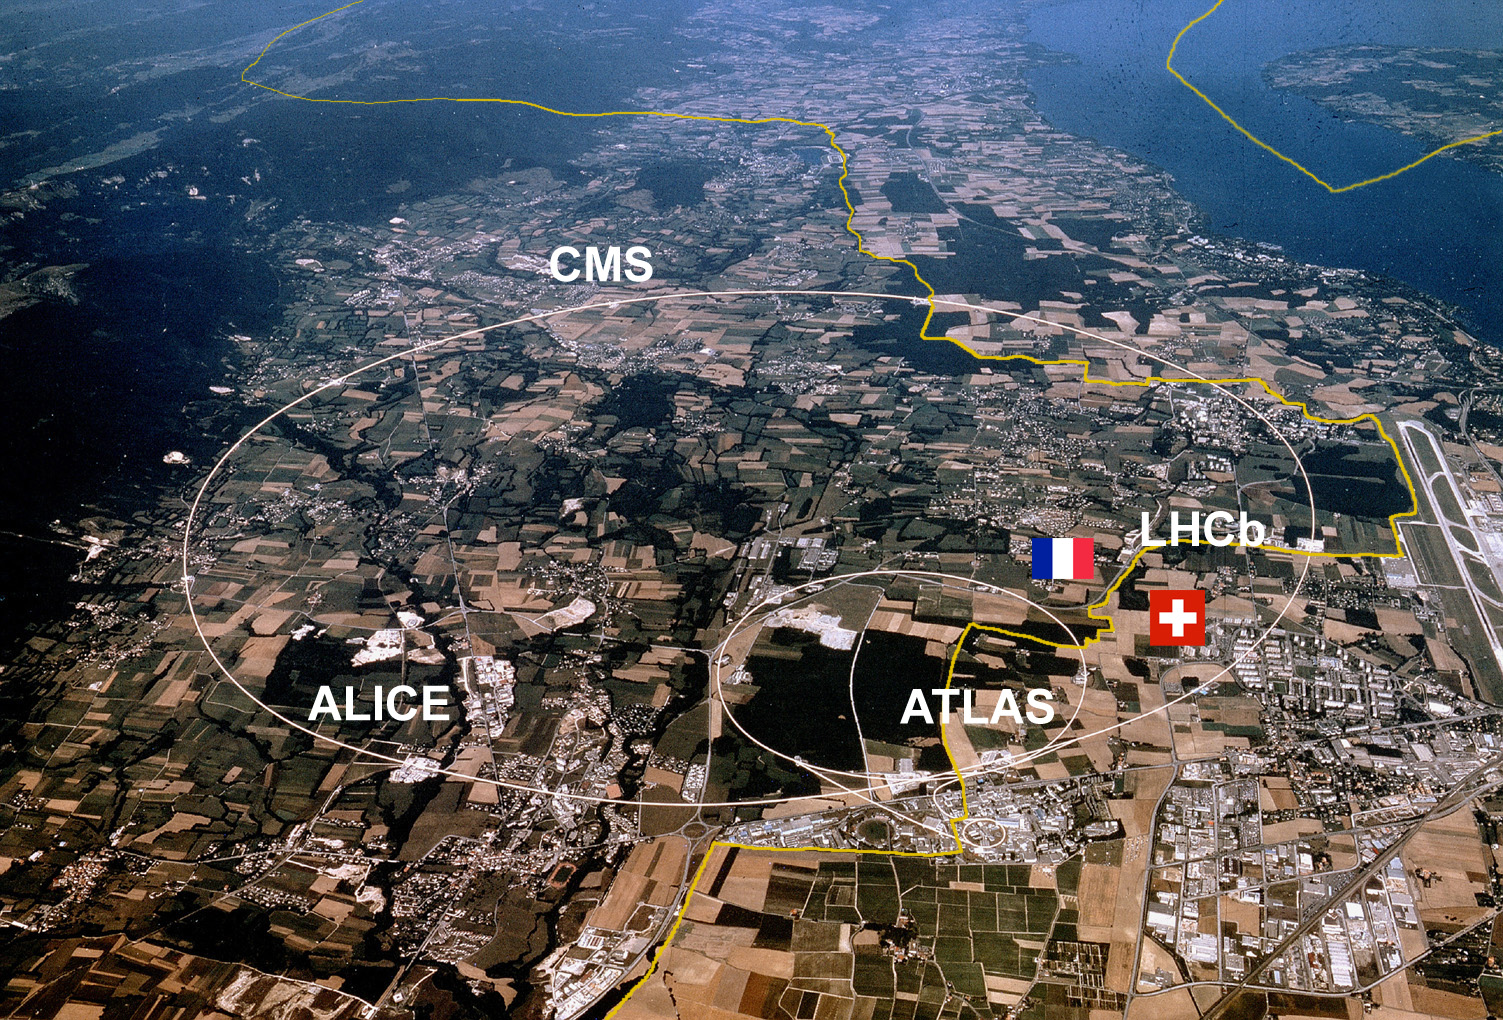
\includegraphics[width=.8\textwidth]{../invisible/TalkPics/cern-lhc-aerial.jpg}
  \end{frame}

  \begin{frame}
    \frametitle{Compact Muon Solenoid (CMS) at the LHC}
    %sheer number of particles and complexity of object reconstruction
    \begin{itemize}
    \item 75M read-out channels just in inner tracker
    \item Has to record a collision every 25ns
    \end{itemize}
    \centering
    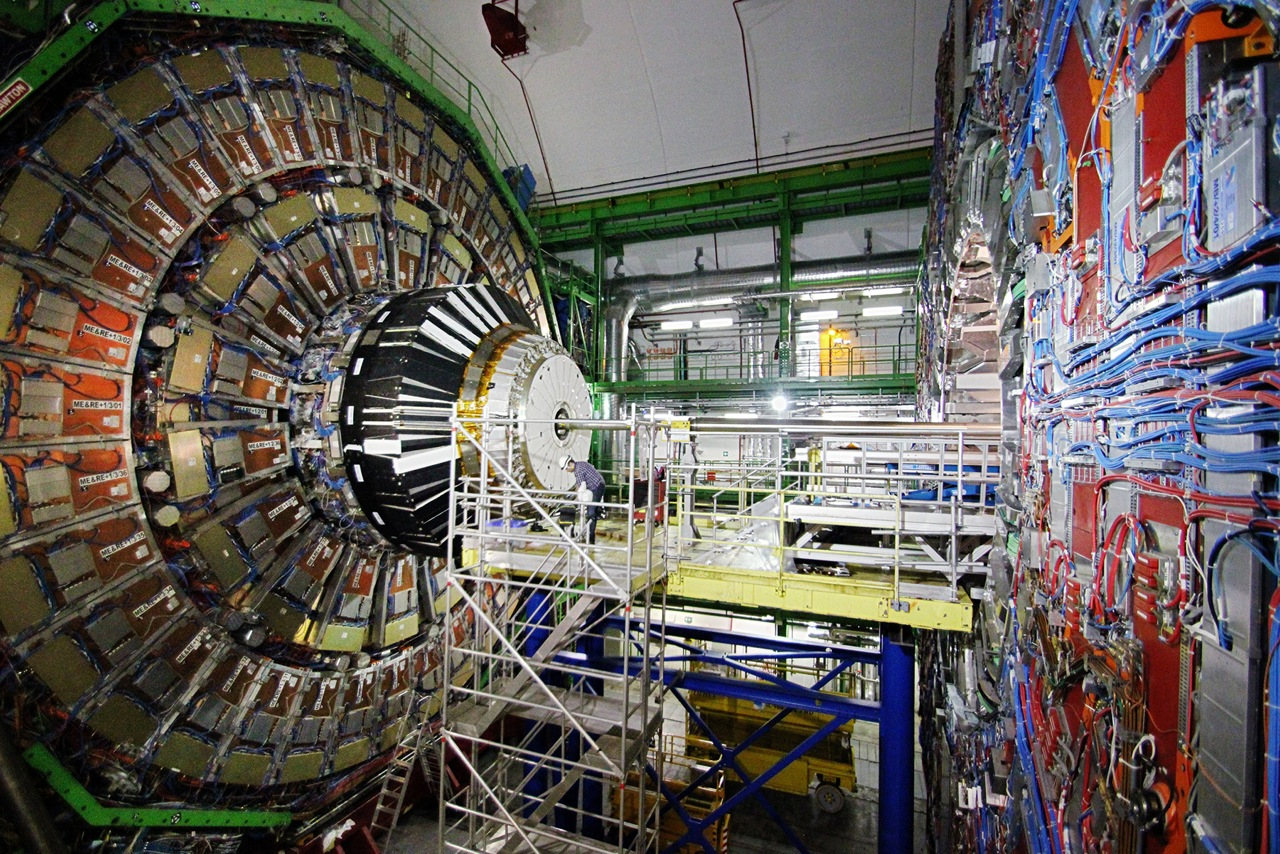
\includegraphics[width=.78\textwidth]{../invisible/TalkPics/sgs120315/cmsphoto.jpeg}
  \end{frame}

  \begin{frame}
    \frametitle{CMS}
    \begin{itemize}
    \item Over 5000 active members from 199 institutes in 46 countries
    \end{itemize}
    
    \centering
    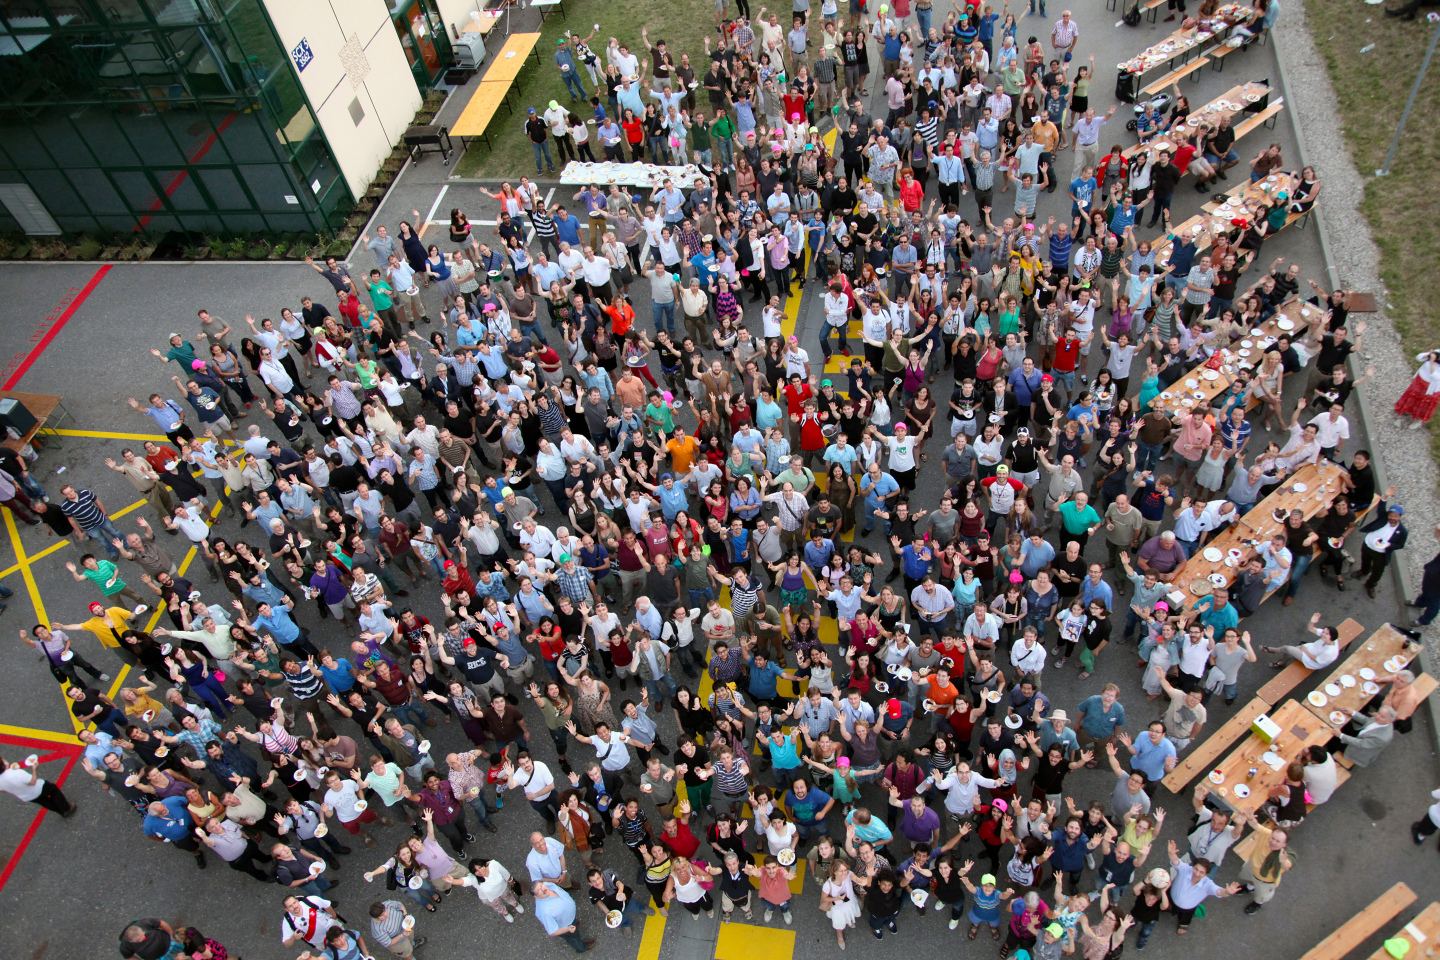
\includegraphics[height=.7\textheight]{TalkPics/ComputationalPhysicsApplications/cmsparty.jpg}
  \end{frame}

  \begin{frame}
    \frametitle{CMS at the LHC}
    %sheer number of particles and complexity of object reconstruction
    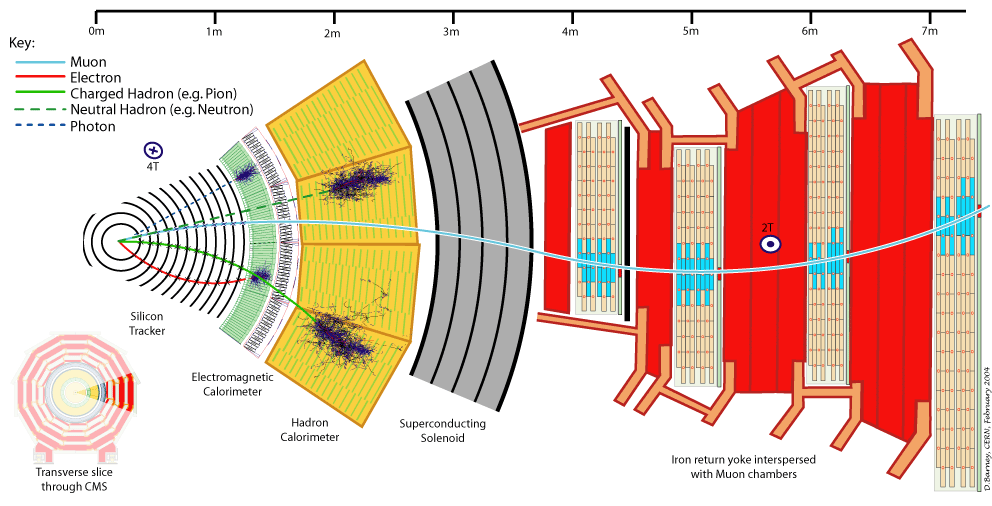
\includegraphics[width=\textwidth]{../invisible/TalkPics/CMS_Slice.png}
  \end{frame}

  \begin{frame}
    \frametitle{Vertex Finding: Simulated Annealing}
    \centering
    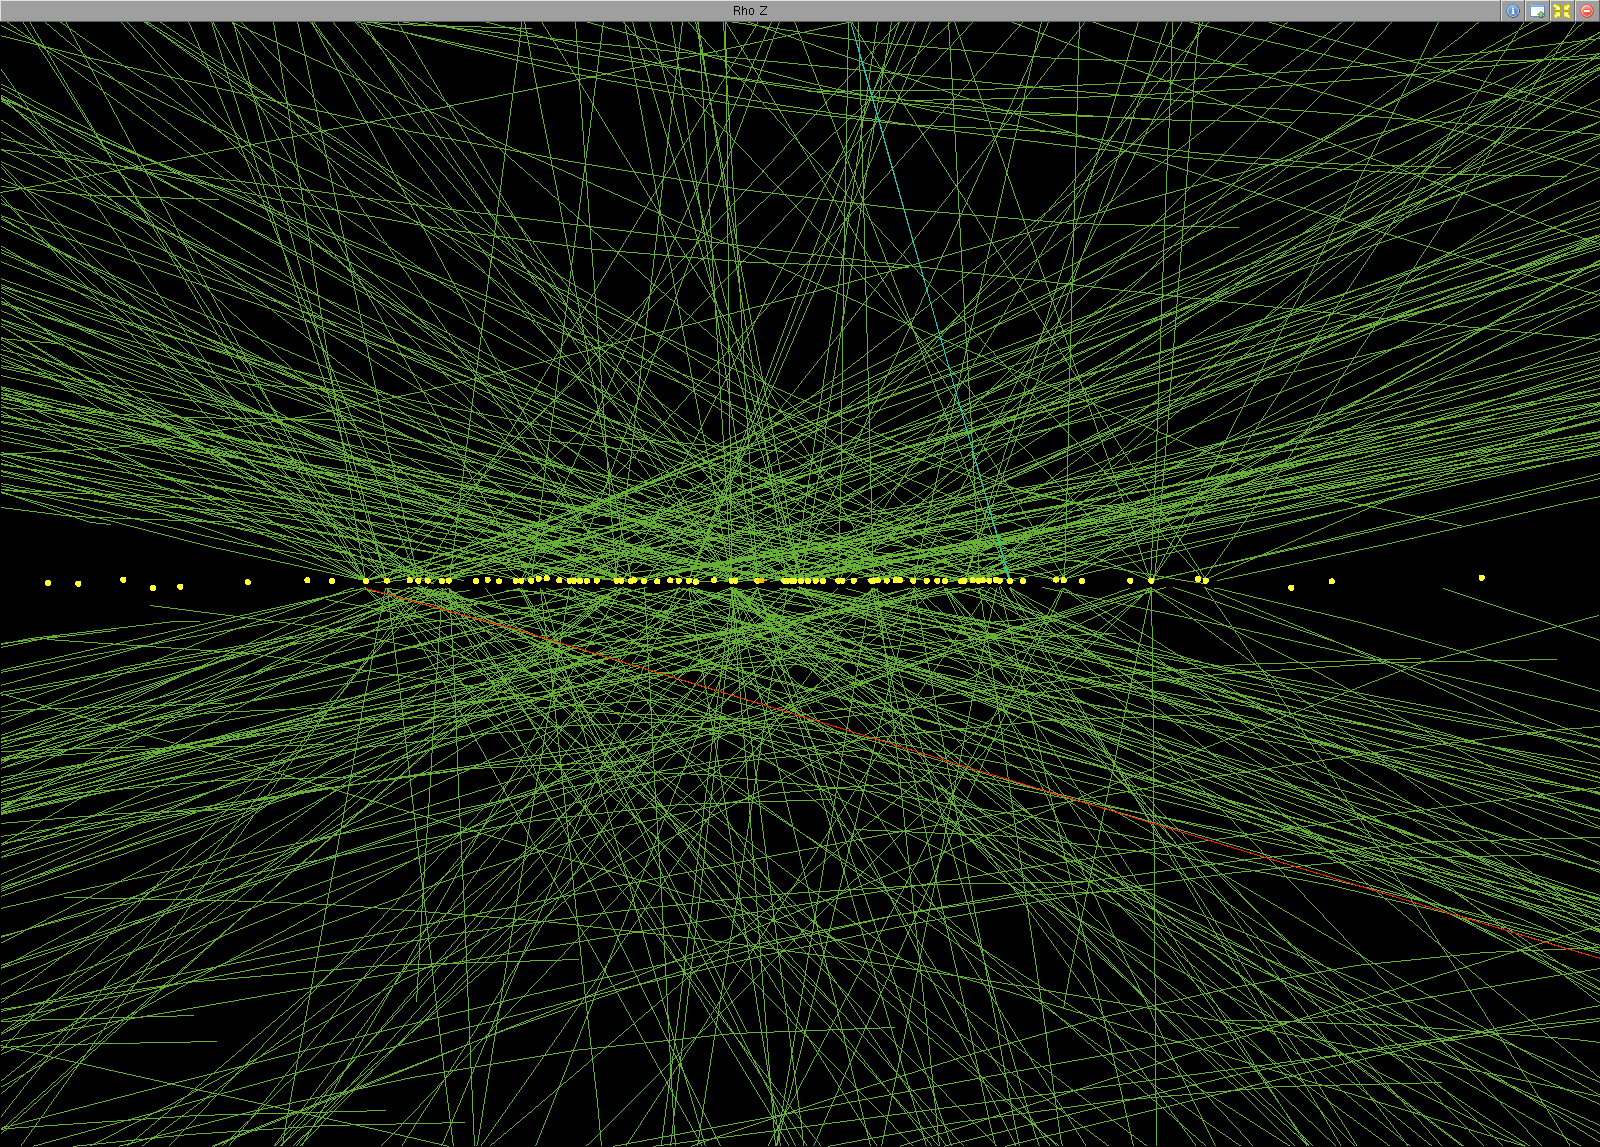
\includegraphics[width=.9\textwidth]{TalkPics/ComputationalPhysicsApplications/cmspvrecon.png}
  \end{frame}

  \begin{frame}
    \frametitle{Vertex Finding: Annealing}
    %??slide 30 lecture 8 for CMS PV finding deterministic annealing
    %??talk through algorithm
    \begin{columns}
      \column{1.1\textwidth}
      \begin{itemize}
      \item Start with a set of tracks with positions $z_{i}$, uncertainty $\sigma_{i}$
      \item Want to find the set of vertex positions $z_{k}$ that they come from
      \item Lots of local minima that you could get stuck in
      \item[-] Good candidate for annealing (see lecture 8)
      \end{itemize}
      \end{columns}
  \end{frame}
  
  \begin{frame}
    \frametitle{Vertex Finding: Annealing}
    \begin{itemize}
    \item Define the `free energy' of the system:
       \begin{equation*}
         F=-T\sum_{i}^{\# tracks}log\sum_{k}^{\# vertices}exp\left[-\frac{1}{T}\frac{\left(z_{i}^{T}-z_{k}^{V}\right)^{2}}{\sigma_{i}^{2}}\right]^{2}
       \end{equation*}
     \item Temperature $T$ defines the penalty for a track being far from a vertex
    \end{itemize}
  \end{frame}

  \begin{frame}
    \frametitle{Vertex Finding: Annealing}
      \begin{itemize}
      \item Start at high $T$ with a single vertex
      \item Find the value of $z_{vertex}$ that minimises F
      \item Reduce $T$ and repeat until the minimum of F turns into a saddle point
      \end{itemize}
      \centering
      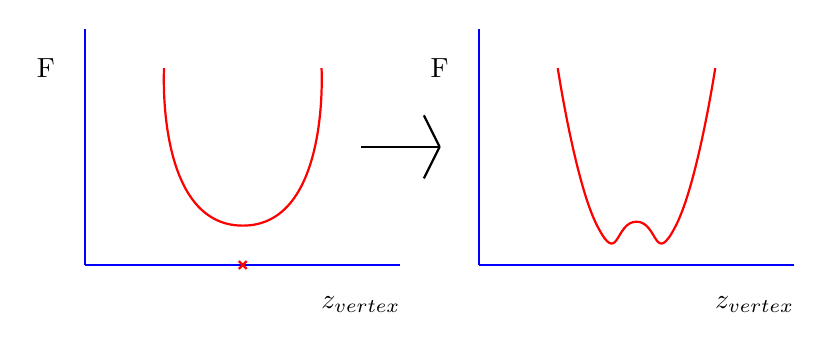
\begin{tikzpicture}[thick]
        %left
        \node at (0.5,2) {F};
        \node at (4.5,-1) {$z_{vertex}$};
        \draw[red] plot [smooth,tension=2] coordinates {(2,2) (3,0) (4,2)};
        \draw[blue] plot [smooth,tension=2] coordinates {(1,-0.5) (5,-0.5)};
        \draw[blue] plot [smooth,tension=2] coordinates {(1,-0.5) (1,2.5)};
        \draw[red] plot [smooth,tension=2] coordinates {(2.95,-0.55) (3.05,-0.45)};
        \draw[red] plot [smooth,tension=2] coordinates {(2.95,-0.45) (3.05,-0.55)};

        \draw[black] plot coordinates {(4.5,1) (5.5,1)};
        \draw[black] plot coordinates {(5.5,1) (5.3,1.4)};
        \draw[black] plot coordinates {(5.5,1) (5.3,0.6)};

        %right
        \node at (5.5,2) {F};
        \node at (9.5,-1) {$z_{vertex}$};
        \draw[red] plot [smooth,tension=1] coordinates {(7,2) (7.5,0.) (8,0.05) (8.5,0) (9,2)};
        \draw[blue] plot [smooth,tension=2] coordinates {(6,-0.5) (10,-0.5)};
        \draw[blue] plot [smooth,tension=2] coordinates {(6,-0.5) (6,2.5)};
        %\draw[red] plot [smooth,tension=2] coordinates {(7.9,-0.55) (8.1,-0.45)};
        %\draw[red] plot [smooth,tension=2] coordinates {(7.9,-0.45) (8.1,-0.55)};
      \end{tikzpicture}
  \end{frame}

  \begin{frame}
    \frametitle{Vertex Finding: Annealing}
      \begin{itemize}
      \item If there's a saddle point split the closest vertex into two
      \item Repeat minimisiation with the new number of vertices
      \item Continue reducing $T$ and repeating until you reach $T_{min}$
      \item Algorithm finds both position and number of vertices
      \end{itemize}
      \centering
      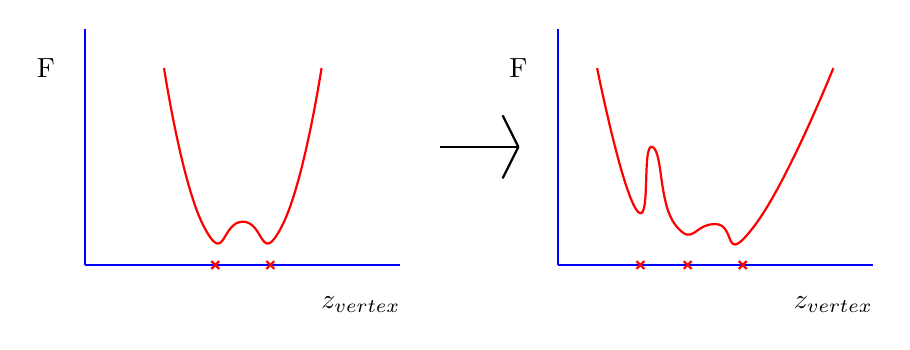
\begin{tikzpicture}[thick]
        %left
        \node at (5.5,2) {F};
        \node at (9.5,-1) {$z_{vertex}$};
        \draw[red] plot [smooth,tension=1] coordinates {(7,2) (7.5,0) (8,0.05) (8.5,0) (9,2)};
        \draw[blue] plot [smooth,tension=2] coordinates {(6,-0.5) (10,-0.5)};
        \draw[blue] plot [smooth,tension=2] coordinates {(6,-0.5) (6,2.5)};
        \draw[red] plot [smooth,tension=2] coordinates {(7.6,-0.55) (7.7,-0.45)};
        \draw[red] plot [smooth,tension=2] coordinates {(7.6,-0.45) (7.7,-0.55)};
        \draw[red] plot [smooth,tension=2] coordinates {(8.3,-0.55) (8.4,-0.45)};
        \draw[red] plot [smooth,tension=2] coordinates {(8.3,-0.45) (8.4,-0.55)};

        \draw[black] plot coordinates {(10.5,1) (11.5,1)};
        \draw[black] plot coordinates {(11.5,1) (11.3,1.4)};
        \draw[black] plot coordinates {(11.5,1) (11.3,0.6)};

        %right
        \node at (11.5,2) {F};
        \node at (15.5,-1) {$z_{vertex}$};
        \draw[red] plot [smooth,tension=1] coordinates {(12.5,2) (13,0.2) (13.2,1) (13.5,0) (14,0.02) (14.5,0) (15.5,2)};
        \draw[blue] plot [smooth,tension=2] coordinates {(12,-0.5) (16,-0.5)};
        \draw[blue] plot [smooth,tension=2] coordinates {(12,-0.5) (12,2.5)};
        \draw[red] plot [smooth,tension=2] coordinates {(13.6,-0.55) (13.7,-0.45)};
        \draw[red] plot [smooth,tension=2] coordinates {(13.6,-0.45) (13.7,-0.55)};
        \draw[red] plot [smooth,tension=2] coordinates {(14.3,-0.55) (14.4,-0.45)};
        \draw[red] plot [smooth,tension=2] coordinates {(14.3,-0.45) (14.4,-0.55)};
        \draw[red] plot [smooth,tension=2] coordinates {(13,-0.55) (13.1,-0.45)};
        \draw[red] plot [smooth,tension=2] coordinates {(13,-0.45) (13.1,-0.55)};
      \end{tikzpicture}
  \end{frame}

  \begin{frame}
    \frametitle{Jet Energy Resolution: Pseudo-Random numbers}
    %??outline what JER is pseudo-random numbers useful for reproducibility e.g. JES/JER calculation for CMS comment on validation
    \begin{columns}
      \column{.5\textwidth}
      \begin{itemize}
      \item A jet is a collimated spray of hadrons
      \item In simulation we assume a certain energy measurement resolution
      \item This is then measured in data and we need to update the simulation
      \end{itemize}
      \column{.5\textwidth}
      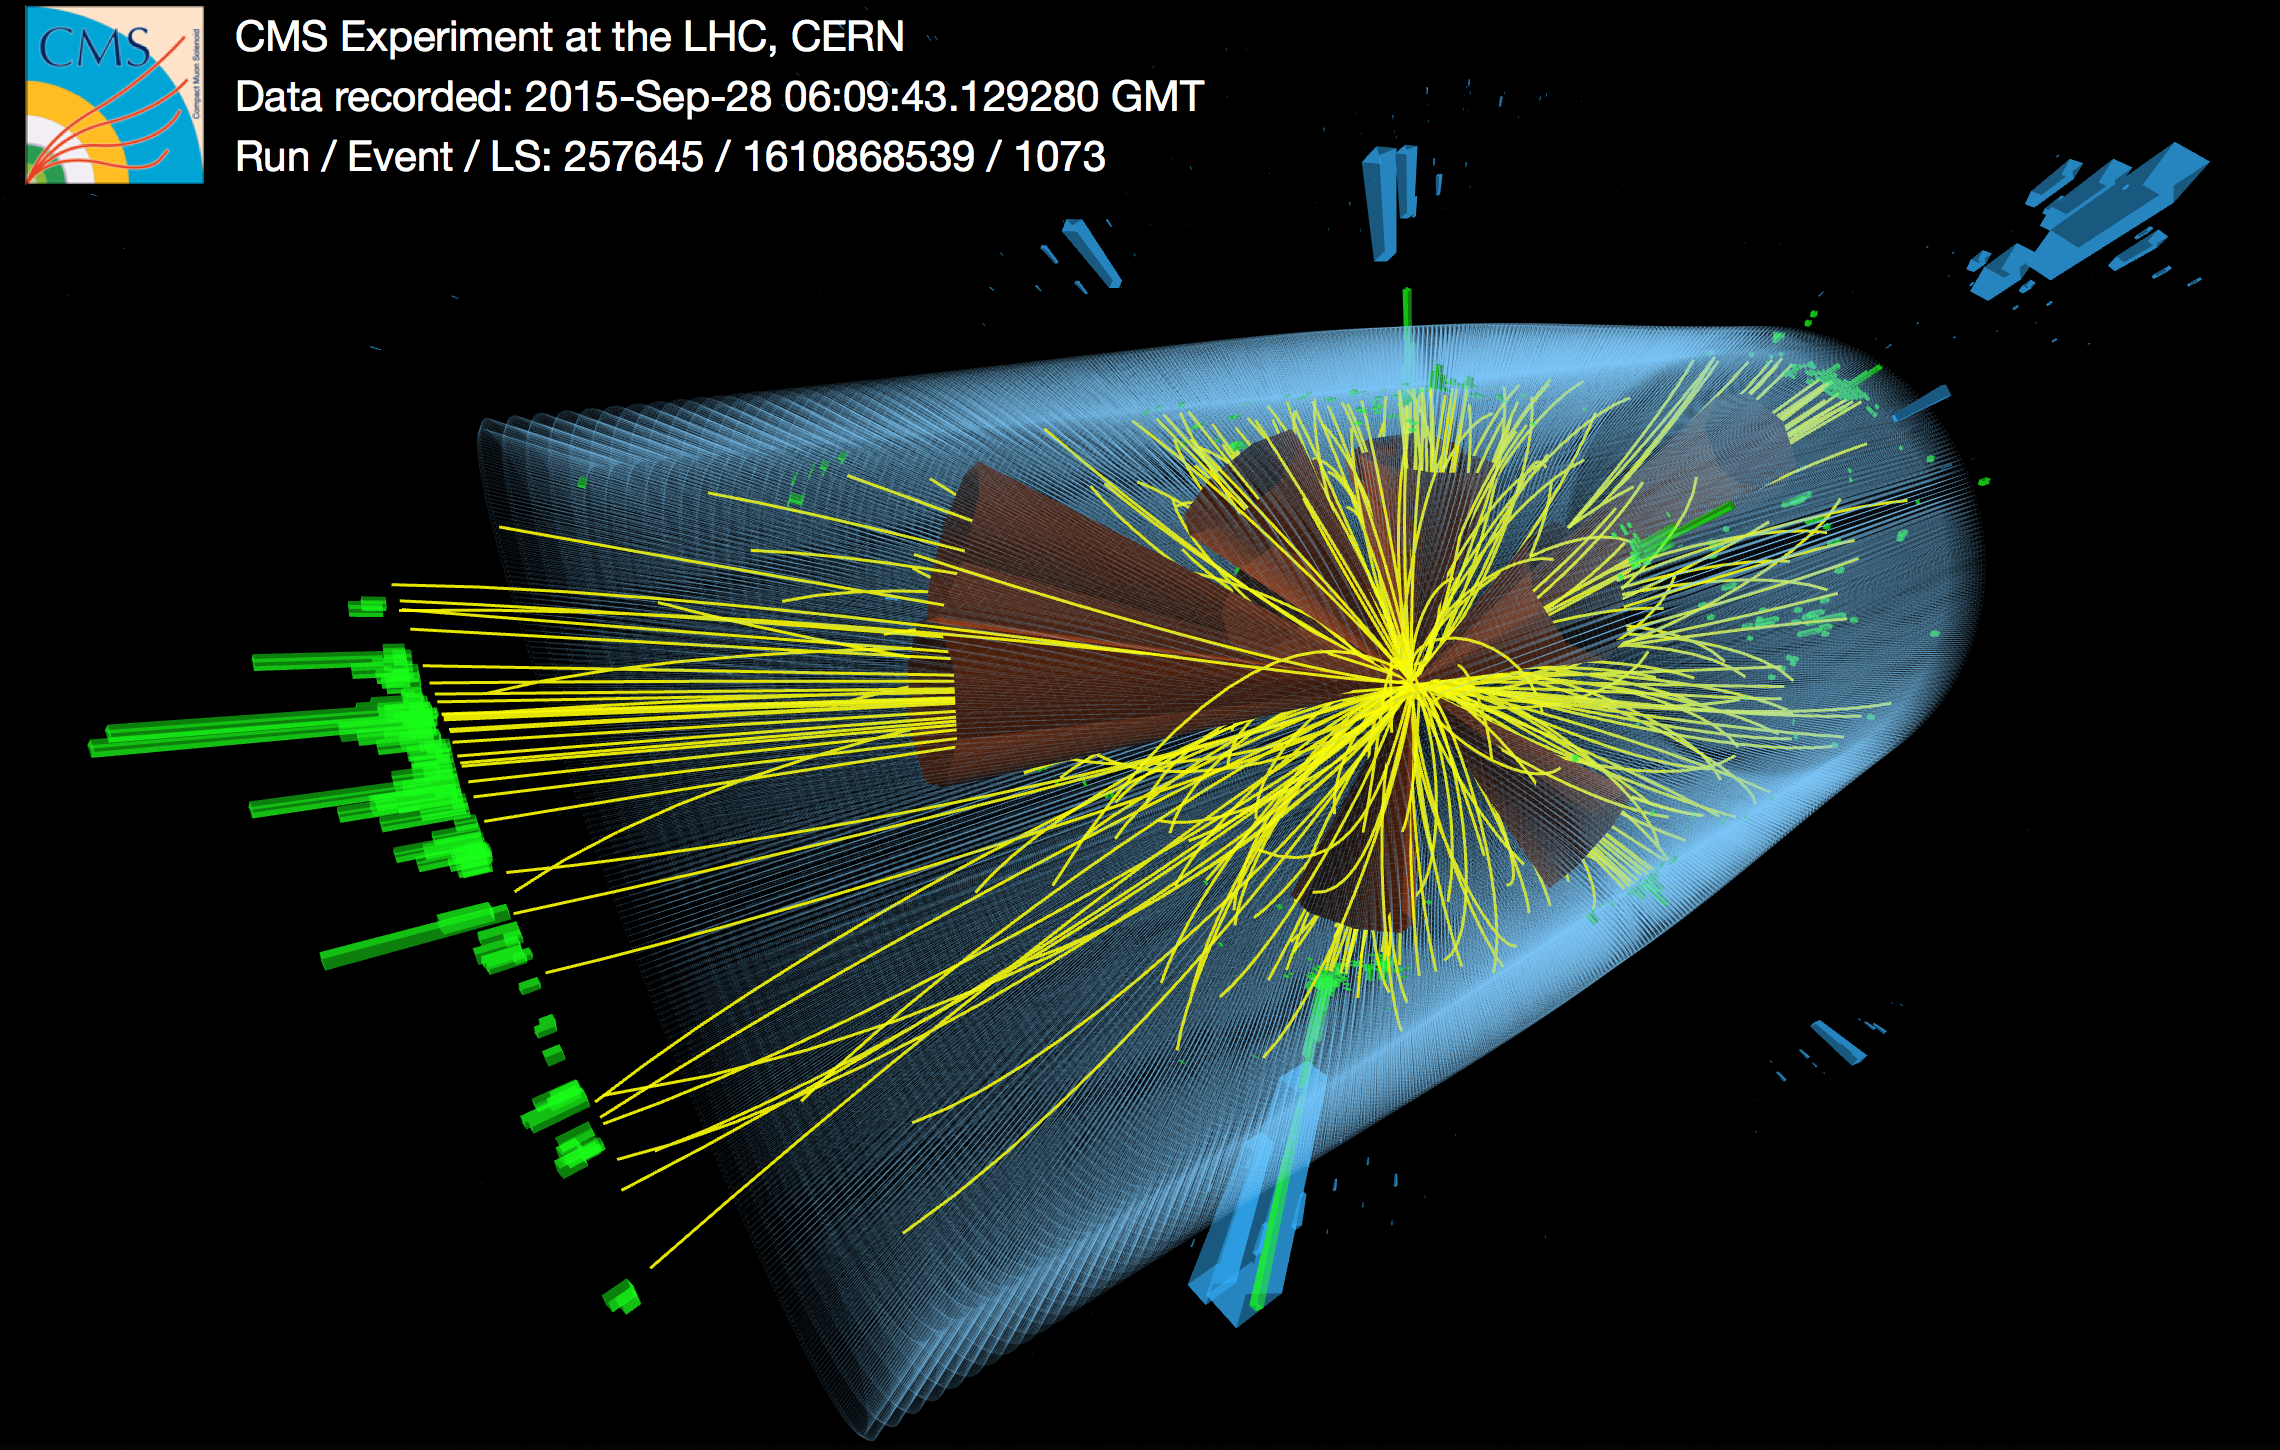
\includegraphics[width=\textwidth]{TalkPics/ComputationalPhysicsApplications/jetevent.png}
    \end{columns}
    
  \end{frame}

  \begin{frame}
    \frametitle{Jet Energy Resolution: Pseudo-Random numbers}
    %??talk about validation and pseudo-random numbers pseudo-random numbers useful for reproducibility e.g. JES/JER calculation for CMS comment on validation
    \begin{itemize}
    \item Usually need to slightly worsen the resolution
    \item Add a random amount of energy drawn from a gaussian with width:
      \begin{equation*}
        \sqrt{c^{2}-1}\sigma_{simulation}
      \end{equation*}
    \item Still want reproducibility for validation against other analysers
    \item[-] Use a pseudorandom number
    \item The framework where this was implemented has 8 active developers and is mostly written in C++
    \end{itemize}
  \end{frame}

%??accept reject from Clarence's NEUT stuff
%??Maybe cholesky decomposition for matrix bit


  \begin{frame}
    \frametitle{Summary}
    \label{lastframe}
    \begin{itemize}
    \item Showed several applications of the techniques from previous lectures
    \item[-] Markov chain Monte Carlo
    \item[-] Simulated annealing
    \item[-] Pseudo-random numbers
    \item Described the scale of the challenges faced in particle physics and the size of the collaborations needed to solve them

    \end{itemize}
  \end{frame}

  %Backup goes here
  
\end{fmffile}
\end{document}

\begin{frame}
\end{frame}
